% Options for packages loaded elsewhere
\PassOptionsToPackage{unicode}{hyperref}
\PassOptionsToPackage{hyphens}{url}
\documentclass[
]{article}
\usepackage{xcolor}
\usepackage{amsmath,amssymb}
\setcounter{secnumdepth}{-\maxdimen} % remove section numbering
\usepackage{iftex}
\ifPDFTeX
  \usepackage[T1]{fontenc}
  \usepackage[utf8]{inputenc}
  \usepackage{textcomp} % provide euro and other symbols
\else % if luatex or xetex
  \usepackage{unicode-math} % this also loads fontspec
  \defaultfontfeatures{Scale=MatchLowercase}
  \defaultfontfeatures[\rmfamily]{Ligatures=TeX,Scale=1}
\fi
\usepackage{lmodern}
\ifPDFTeX\else
  % xetex/luatex font selection
\fi
% Use upquote if available, for straight quotes in verbatim environments
\IfFileExists{upquote.sty}{\usepackage{upquote}}{}
\IfFileExists{microtype.sty}{% use microtype if available
  \usepackage[]{microtype}
  \UseMicrotypeSet[protrusion]{basicmath} % disable protrusion for tt fonts
}{}
\makeatletter
\@ifundefined{KOMAClassName}{% if non-KOMA class
  \IfFileExists{parskip.sty}{%
    \usepackage{parskip}
  }{% else
    \setlength{\parindent}{0pt}
    \setlength{\parskip}{6pt plus 2pt minus 1pt}}
}{% if KOMA class
  \KOMAoptions{parskip=half}}
\makeatother
\usepackage{color}
\usepackage{fancyvrb}
\newcommand{\VerbBar}{|}
\newcommand{\VERB}{\Verb[commandchars=\\\{\}]}
\DefineVerbatimEnvironment{Highlighting}{Verbatim}{commandchars=\\\{\}}
% Add ',fontsize=\small' for more characters per line
\newenvironment{Shaded}{}{}
\newcommand{\AlertTok}[1]{\textcolor[rgb]{1.00,0.00,0.00}{\textbf{#1}}}
\newcommand{\AnnotationTok}[1]{\textcolor[rgb]{0.38,0.63,0.69}{\textbf{\textit{#1}}}}
\newcommand{\AttributeTok}[1]{\textcolor[rgb]{0.49,0.56,0.16}{#1}}
\newcommand{\BaseNTok}[1]{\textcolor[rgb]{0.25,0.63,0.44}{#1}}
\newcommand{\BuiltInTok}[1]{\textcolor[rgb]{0.00,0.50,0.00}{#1}}
\newcommand{\CharTok}[1]{\textcolor[rgb]{0.25,0.44,0.63}{#1}}
\newcommand{\CommentTok}[1]{\textcolor[rgb]{0.38,0.63,0.69}{\textit{#1}}}
\newcommand{\CommentVarTok}[1]{\textcolor[rgb]{0.38,0.63,0.69}{\textbf{\textit{#1}}}}
\newcommand{\ConstantTok}[1]{\textcolor[rgb]{0.53,0.00,0.00}{#1}}
\newcommand{\ControlFlowTok}[1]{\textcolor[rgb]{0.00,0.44,0.13}{\textbf{#1}}}
\newcommand{\DataTypeTok}[1]{\textcolor[rgb]{0.56,0.13,0.00}{#1}}
\newcommand{\DecValTok}[1]{\textcolor[rgb]{0.25,0.63,0.44}{#1}}
\newcommand{\DocumentationTok}[1]{\textcolor[rgb]{0.73,0.13,0.13}{\textit{#1}}}
\newcommand{\ErrorTok}[1]{\textcolor[rgb]{1.00,0.00,0.00}{\textbf{#1}}}
\newcommand{\ExtensionTok}[1]{#1}
\newcommand{\FloatTok}[1]{\textcolor[rgb]{0.25,0.63,0.44}{#1}}
\newcommand{\FunctionTok}[1]{\textcolor[rgb]{0.02,0.16,0.49}{#1}}
\newcommand{\ImportTok}[1]{\textcolor[rgb]{0.00,0.50,0.00}{\textbf{#1}}}
\newcommand{\InformationTok}[1]{\textcolor[rgb]{0.38,0.63,0.69}{\textbf{\textit{#1}}}}
\newcommand{\KeywordTok}[1]{\textcolor[rgb]{0.00,0.44,0.13}{\textbf{#1}}}
\newcommand{\NormalTok}[1]{#1}
\newcommand{\OperatorTok}[1]{\textcolor[rgb]{0.40,0.40,0.40}{#1}}
\newcommand{\OtherTok}[1]{\textcolor[rgb]{0.00,0.44,0.13}{#1}}
\newcommand{\PreprocessorTok}[1]{\textcolor[rgb]{0.74,0.48,0.00}{#1}}
\newcommand{\RegionMarkerTok}[1]{#1}
\newcommand{\SpecialCharTok}[1]{\textcolor[rgb]{0.25,0.44,0.63}{#1}}
\newcommand{\SpecialStringTok}[1]{\textcolor[rgb]{0.73,0.40,0.53}{#1}}
\newcommand{\StringTok}[1]{\textcolor[rgb]{0.25,0.44,0.63}{#1}}
\newcommand{\VariableTok}[1]{\textcolor[rgb]{0.10,0.09,0.49}{#1}}
\newcommand{\VerbatimStringTok}[1]{\textcolor[rgb]{0.25,0.44,0.63}{#1}}
\newcommand{\WarningTok}[1]{\textcolor[rgb]{0.38,0.63,0.69}{\textbf{\textit{#1}}}}
\usepackage{longtable,booktabs,array}
\newcounter{none} % for unnumbered tables
\usepackage{calc} % for calculating minipage widths
% Correct order of tables after \paragraph or \subparagraph
\usepackage{etoolbox}
\makeatletter
\patchcmd\longtable{\par}{\if@noskipsec\mbox{}\fi\par}{}{}
\makeatother
% Allow footnotes in longtable head/foot
\IfFileExists{footnotehyper.sty}{\usepackage{footnotehyper}}{\usepackage{footnote}}
\makesavenoteenv{longtable}
\usepackage{graphicx}
\makeatletter
\newsavebox\pandoc@box
\newcommand*\pandocbounded[1]{% scales image to fit in text height/width
  \sbox\pandoc@box{#1}%
  \Gscale@div\@tempa{\textheight}{\dimexpr\ht\pandoc@box+\dp\pandoc@box\relax}%
  \Gscale@div\@tempb{\linewidth}{\wd\pandoc@box}%
  \ifdim\@tempb\p@<\@tempa\p@\let\@tempa\@tempb\fi% select the smaller of both
  \ifdim\@tempa\p@<\p@\scalebox{\@tempa}{\usebox\pandoc@box}%
  \else\usebox{\pandoc@box}%
  \fi%
}
% Set default figure placement to htbp
\def\fps@figure{htbp}
\makeatother
\setlength{\emergencystretch}{3em} % prevent overfull lines
\providecommand{\tightlist}{%
  \setlength{\itemsep}{0pt}\setlength{\parskip}{0pt}}
\usepackage{bookmark}
\IfFileExists{xurl.sty}{\usepackage{xurl}}{} % add URL line breaks if available
\urlstyle{same}
\hypersetup{
  hidelinks,
  pdfcreator={LaTeX via pandoc}}

\author{}
\date{}

\begin{document}

\section{\texorpdfstring{\textbf{Monte Carlo Simulation of a Simple
Polymer
Chain}}{Monte Carlo Simulation of a Simple Polymer Chain}}\label{monte-carlo-simulation-of-a-simple-polymer-chain}

12 April 2026

\subsection{\texorpdfstring{Team
\textbf{Project\_2026\_II}}{Team Project\_2026\_II}}\label{team-project_2026_ii}

{\def\LTcaptype{none} % do not increment counter
\begin{longtable}[]{@{}
  >{\raggedright\arraybackslash}p{(\linewidth - 6\tabcolsep) * \real{0.0645}}
  >{\raggedright\arraybackslash}p{(\linewidth - 6\tabcolsep) * \real{0.0968}}
  >{\raggedright\arraybackslash}p{(\linewidth - 6\tabcolsep) * \real{0.3710}}
  >{\raggedright\arraybackslash}p{(\linewidth - 6\tabcolsep) * \real{0.4677}}@{}}
\toprule\noalign{}
\begin{minipage}[b]{\linewidth}\raggedright
Name
\end{minipage} & \begin{minipage}[b]{\linewidth}\raggedright
Github
\end{minipage} & \begin{minipage}[b]{\linewidth}\raggedright
Files (Principal Author)
\end{minipage} & \begin{minipage}[b]{\linewidth}\raggedright
Parallelization Contributions
\end{minipage} \\
\midrule\noalign{}
\endhead
\bottomrule\noalign{}
\endlastfoot
MANEL DÍAZ CALVO & ManelDC55 & Monte Carlo, qsub script, Plotting* &
Equilibration Optimization \\
OLIWIER MISZTAL & omisztal & Energy, Shell Scripts, Plotting* & Energy
Calculations \\
ITXASO MUÑOZ ALDALUR & itxasoma & Initial Configurations, Shell Scripts,
File I/O, Plotting* & Independent Replicas, Orchestrator
Read/Broadcasting, Trajectory Parsing \\
ARTHUR IAN MURPHY (\emph{Project Leader}) & ai-murphy & Makefile, Main,
Observables, Plotting* & Ensemble Averaging \\
\end{longtable}
}

\subsection{Project Overview}\label{project-overview}

In this assignment, our goal was to develop a Monte Carlo simulation
program to explore the conformational landscape of a 500-Carbon linear
polymer chain (polyethylene) with varying torsional angles. The
simulation generates the initial conformation (with \& without
Hydrogens), measures torsional energy rotations, end-to-end distance,
and intramolecular Lennard-Jones interactions, and finally analyzes \&
visualizes the results.

After creating a serial processing version of the program,
parallelization techniques involving both MPI and OpenMP were
incorporated. These were compared to the serial version to demonstrate
both their individual and combined High Performance Computing
capabilities \& benefits.

Many techniques taught in class were crucial in the development of this
program, including: - \textbf{Git/Github} as a code respository \&
teamwork coordination platform - \textbf{Makefile} to automate the
compilation and execution of the code - \textbf{Shell scripting} for
facilitating server deployment - \textbf{MPI \& openMP} to parallelize
the code - \textbf{Python} for post-processing and plotting

\subsection{Repository Structure}\label{repository-structure}

Github was used as our team's code repository management system, and
from the root of
\href{https://github.com/Eines-Informatiques-Avancades/Project_2026_II}{the
project}, the code is divided among 3 main folders: \texttt{src},
\texttt{results}, and \texttt{docs}.

\begin{itemize}
\tightlist
\item
  \texttt{src} contains:

  \begin{itemize}
  \tightlist
  \item
    Makefile \& shell scripts
  \item
    Various versions of the main program (serial \& parallel)
  \item
    A \texttt{confs} folder where initial configurations are stored and
    compile-time options can be controlled via a file called
    \texttt{input.dat}
  \item
    A \texttt{lib} folder where module source files, python analysis
    files, and plotting style dependencies reside (\emph{further detail
    below})
  \end{itemize}
\item
  \texttt{results} contains the output data from the simulations
\item
  \texttt{docs} contains documentation and reports, including
  \texttt{img} folder for embedded images
\end{itemize}

In addition to these folders, a customary \texttt{README} file is
included in the root directory detailing run instructions and code
dependencies/requirements. The bulk of the code is written in Fortran,
while the post-processing is done in Python.

\#\#\# Module Library Introduction The following modules support the
\emph{\texttt{main...f90}} files: - \texttt{energy.f90} \&
\texttt{energy\_all\_atoms.f90} - Permit \textbf{dual energy modes},
computing energetic contributions using either TraPPE-UA or OPLS-AA
(with effective backbone potentials) depending on the
\texttt{explicit\_h} toggle dynamically read from \texttt{input.dat}. -
\texttt{initial-conf.f90} - Generates initial configuration of the
polymer chain. - \texttt{io.f90} - File input/ouput module. -
\texttt{monte\_carlo.f90} - Provides the rotation algorithm and
subroutine MCS step used to update spatial configurations. -
\texttt{observables.f90} - Computes the structural observables:
End-to-end distance (\(R_{ee}\)), Radius of Gyration (\(R_g\)), and
torsion angles. - \texttt{parameters.f90} - Stores global parameters
abstracted from \emph{\texttt{main...f90}} code. Works in tandem with
\texttt{input.dat} settings. - \emph{\texttt{plot\_...py}} files -
Various scripts used for plotting observables and serial vs parallel
code comparisons. - \texttt{requirements.txt} - List of python module
dependencies. - \texttt{science.mplstyle} - stylized document used in
plotting to control visualization theme.

\subsection{Code Management via
Github}\label{code-management-via-github}

The project leader was responsible for reviewing all pull requests,
ensuring that the code followed the project guidelines, and merging the
code into the main branch. The team coordinated through a WhatsApp group
chat and would regularly check in on each other's progress. Everyone was
informed when code was merged so we could all pull the latest changes.

Most times, approving and merging was straightforward with no issues,
but there was an interesting challenge when multiple uploads from
different team members overlapped, causing conflicts. This forced us to
learn about stashing and rebasing to the newly updated master branch
before recommitting. The following process was ironed out to ensure a
smooth integration:

\begin{enumerate}
\def\labelenumi{\arabic{enumi}.}
\item
  Stash local (uncommitted) changes

\begin{Shaded}
\begin{Highlighting}[]
   \FunctionTok{git}\NormalTok{ stash}
\end{Highlighting}
\end{Shaded}
\item
  Pull latest changes from master branch

\begin{Shaded}
\begin{Highlighting}[]
   \FunctionTok{git}\NormalTok{ checkout master}
   \FunctionTok{git}\NormalTok{ pull main master}
\end{Highlighting}
\end{Shaded}
\item
  Rebase local changes onto master branch so it starts after the new
  merged code

\begin{Shaded}
\begin{Highlighting}[]
   \FunctionTok{git}\NormalTok{ checkout }\OperatorTok{\textless{}}\NormalTok{fork{-}feature}\OperatorTok{\textgreater{}}\NormalTok{/}\OperatorTok{\textless{}}\NormalTok{fork{-}branch}\OperatorTok{\textgreater{}}
   \FunctionTok{git}\NormalTok{ rebase master}
\end{Highlighting}
\end{Shaded}
\item
  Resolve any conflicts \& re-apply stashed changes

\begin{Shaded}
\begin{Highlighting}[]
   \FunctionTok{git}\NormalTok{ stash pop}
\end{Highlighting}
\end{Shaded}
\item
  Commit and push (using \texttt{-\/-force} parameter due to rebase)

\begin{Shaded}
\begin{Highlighting}[]
   \FunctionTok{git}\NormalTok{ push }\OperatorTok{\textless{}}\NormalTok{fork{-}remote}\OperatorTok{\textgreater{}} \OperatorTok{\textless{}}\NormalTok{fork{-}branch}\OperatorTok{\textgreater{}}\NormalTok{ {-}{-}force}
\end{Highlighting}
\end{Shaded}
\end{enumerate}

\subsection{Makefile}\label{makefile}

As the project evolved, so did the Makefile. Here are some of the
features we implemented:

Starting off, there are few main variables that control the compilation
process.

\begin{Shaded}
\begin{Highlighting}[]
\DataTypeTok{FC}       \CharTok{=}\StringTok{ gfortran}
\DataTypeTok{FFLAGS}   \CharTok{=}\StringTok{ {-}O2 {-}Wall {-}Wextra}
\DataTypeTok{OBJ\_DIR}  \CharTok{=}\StringTok{ ../bin}
\DataTypeTok{EXE}      \CharTok{=}\StringTok{ }\CharTok{$(}\DataTypeTok{OBJ\_DIR}\CharTok{)}\StringTok{/main\_serial.x}
\DataTypeTok{LIB\_OBJ}  \CharTok{=}\StringTok{ }\CharTok{$(}\DataTypeTok{OBJ\_DIR}\CharTok{)}\StringTok{/parameters.o }\CharTok{\textbackslash{}}
\StringTok{           }\CharTok{$(}\DataTypeTok{OBJ\_DIR}\CharTok{)}\StringTok{/io.o }\CharTok{\textbackslash{}}
\StringTok{           ...}
\DataTypeTok{MAIN\_OBJ} \CharTok{=}\StringTok{ }\CharTok{$(}\DataTypeTok{OBJ\_DIR}\CharTok{)}\StringTok{/main\_serial.o}

\DataTypeTok{NP}          \CharTok{?=}\StringTok{ 4}
\DataTypeTok{OMP\_THREADS} \CharTok{?=}\StringTok{ 2}
\end{Highlighting}
\end{Shaded}

\begin{itemize}
\tightlist
\item
  \texttt{FC}: Stands for ``Fortran Compiler''. We tell it to use
  gfortran.
\item
  \texttt{FFLAGS}: These are the compiler flags. \texttt{-O2} is the
  optimization schema, and \texttt{-Wall\ -Wextra} enables warnings.
\item
  \texttt{OBJ\_DIR} \& \texttt{EXE}: Defines the compiled binaries
  directory and the name of the final executable.
\item
  \texttt{LIB\_OBJ} \& \texttt{MAIN\_OBJ}: Defines the object files for
  the library and the main program.
\item
  \texttt{NP} \& \texttt{OMP\_THREADS}: Defines the number of processes
  (MPI) and threads (openMP) to use for the parallel version of the
  program. The default values are set to 4 and 2, respectively, but they
  can be overridden by setting them when compiling in the command line
  (e.g., \texttt{make\ run\_parallel\ NP=7\ OMP\_THREADS=3}).
\end{itemize}

In order to encompass both the serial and parallel versions of the
program, a check is performed on the \texttt{make} command entered on
the command-line for the word \texttt{parallel}. If found, the user's
system is searched to ensure the environment has the necessary MPI and
OpenMP libraries installed. If not, an error message is printed and the
program exits. If they are installed, the compiler variable \texttt{FC}
is overwritten and the MPI and OpenMP flags are added to the
\texttt{FFLAGS} variable.

\begin{Shaded}
\begin{Highlighting}[]
\ControlFlowTok{ifneq}\NormalTok{ (,}\CharTok{$(}\KeywordTok{findstring}\StringTok{ parallel}\KeywordTok{,}\CharTok{$(}\DataTypeTok{MAKECMDGOALS}\CharTok{))}\NormalTok{)}
  \CommentTok{\# MPI Compiler Wrapper Verification}
  \DataTypeTok{MPI\_BIN} \CharTok{:=}\StringTok{ }\CharTok{$(}\KeywordTok{shell}\StringTok{ command {-}v mpif90 2\textgreater{}/dev/null}\CharTok{)}
  \ControlFlowTok{ifeq}\NormalTok{ (}\CharTok{$(}\KeywordTok{strip}\StringTok{ }\CharTok{$(}\DataTypeTok{MPI\_BIN}\CharTok{))}\NormalTok{,)}
    \CharTok{$(}\KeywordTok{error}\StringTok{ "MPI Compiler is required but \textquotesingle{}mpif90\textquotesingle{} was not found! Please install it (e.g. \textquotesingle{}sudo apt install openmpi{-}bin\textquotesingle{})"}\CharTok{)}
  \ControlFlowTok{endif}
  \CommentTok{\# Overwrite Compiler for MPI parallelization flag linking}
  \DataTypeTok{FC} \CharTok{=}\StringTok{ mpif90}
\NormalTok{  ...}
\end{Highlighting}
\end{Shaded}

Instead of writing a rule for every single \texttt{.f90} file, a pattern
rule (with \texttt{\%}) is used.

\begin{Shaded}
\begin{Highlighting}[]
\DecValTok{$(OBJ\_DIR)/\%.o:}\DataTypeTok{ lib/\%.f90}
\ErrorTok{    }\CharTok{@}\FunctionTok{mkdir {-}p }\CharTok{$(}\DataTypeTok{OBJ\_DIR}\CharTok{)}
    \CharTok{$(}\DataTypeTok{FC}\CharTok{)} \CharTok{$(}\DataTypeTok{FFLAGS}\CharTok{)}\NormalTok{ {-}J}\CharTok{$(}\DataTypeTok{OBJ\_DIR}\CharTok{)}\NormalTok{ {-}I}\CharTok{$(}\DataTypeTok{OBJ\_DIR}\CharTok{)}\NormalTok{ {-}c }\CharTok{$\textless{}}\NormalTok{ {-}o }\CharTok{$@}
\end{Highlighting}
\end{Shaded}

\begin{itemize}
\tightlist
\item
  It says: ``To make any \texttt{.o} file in the object directory
  (\texttt{bin/}) from a matching \texttt{.f90} file in \texttt{lib/},
  run this command.''
\item
  \texttt{-c\ \$\textless{}}: Compiles the ``first dependency''
  (\texttt{\$\textless{}}, which is the \texttt{.f90} file) without
  linking (because that's done in the \texttt{\$(EXE)} target).
\item
  \texttt{-J\$(OBJ\_DIR)\ -I\$(OBJ\_DIR)}: Tells Fortran to put module
  \texttt{.mod} files in the \texttt{bin/} folder.
\end{itemize}

The following is an example of the \texttt{all} target (serial version
of the program) with its executable structure, which we then follow up
with the explicit dependencies to create the \texttt{.o} files for the
library modules and the main program

\begin{Shaded}
\begin{Highlighting}[]
\DecValTok{all:}\DataTypeTok{ }\CharTok{$(}\DataTypeTok{EXE}\CharTok{)}

\DecValTok{$(EXE):}\DataTypeTok{ }\CharTok{$(}\DataTypeTok{LIB\_OBJ}\CharTok{)}\DataTypeTok{ }\CharTok{$(}\DataTypeTok{MAIN\_OBJ}\CharTok{)}
\ErrorTok{    }\CharTok{@}\FunctionTok{mkdir {-}p }\CharTok{$(}\DataTypeTok{OBJ\_DIR}\CharTok{)}
    \CharTok{$(}\DataTypeTok{FC}\CharTok{)} \CharTok{$(}\DataTypeTok{FFLAGS}\CharTok{)}\NormalTok{ {-}o }\CharTok{$@} \CharTok{$(}\DataTypeTok{LIB\_OBJ}\CharTok{)} \CharTok{$(}\DataTypeTok{MAIN\_OBJ}\CharTok{)}

\DecValTok{$(OBJ\_DIR)/energy.o:}\DataTypeTok{ lib/energy.f90 }\CharTok{\textbackslash{}}
\DataTypeTok{                     }\CharTok{$(}\DataTypeTok{OBJ\_DIR}\CharTok{)}\DataTypeTok{/parameters.o}
\NormalTok{...}

\DecValTok{$(OBJ\_DIR)/main\_serial.o:}\DataTypeTok{ main\_serial.f90 }\CharTok{$(}\DataTypeTok{LIB\_OBJ}\CharTok{)}
\ErrorTok{    }\CharTok{@}\FunctionTok{mkdir {-}p }\CharTok{$(}\DataTypeTok{OBJ\_DIR}\CharTok{)}
    \CharTok{$(}\DataTypeTok{FC}\CharTok{)} \CharTok{$(}\DataTypeTok{FFLAGS}\CharTok{)}\NormalTok{ {-}J}\CharTok{$(}\DataTypeTok{OBJ\_DIR}\CharTok{)}\NormalTok{ {-}I}\CharTok{$(}\DataTypeTok{OBJ\_DIR}\CharTok{)}\NormalTok{ {-}c }\CharTok{$\textless{}}\NormalTok{ {-}o }\CharTok{$@}
\end{Highlighting}
\end{Shaded}

\begin{itemize}
\tightlist
\item
  \texttt{all}: This is the default target that needs \texttt{\$(EXE)}
  to exist.
\item
  \texttt{\$(EXE)}: To build the final executable, it needs all the .o
  files from the \texttt{../bin} folder, which it makes sure exists
  (\texttt{mkdir\ -p}), and then links them all together using
  \texttt{gfortran} or \texttt{mpif90} to output (\texttt{-o\ \$@}) the
  final program.

  \begin{itemize}
  \tightlist
  \item
    \textbf{Note}: The \texttt{@} symbol is used 2 different ways here:

    \begin{enumerate}
    \def\labelenumi{\arabic{enumi}.}
    \tightlist
    \item
      Before the \texttt{mkdir} command to suppress being printed to the
      terminal.
    \item
      As an automatic variable representing the target name
      (\texttt{\$(EXE)} in this case).
    \end{enumerate}
  \end{itemize}
\end{itemize}

Last, we declare the shortcut commands as \texttt{.PHONY} targets to
prevent conflicts with files that may have the same name as a target.

\begin{Shaded}
\begin{Highlighting}[]
\OtherTok{.PHONY:}\DataTypeTok{ all clean run figures pipeline}

\DecValTok{run:}\DataTypeTok{ all}
\ErrorTok{    }\CharTok{@}\FunctionTok{mkdir {-}p ../results}
    \CharTok{$(}\DataTypeTok{EXE}\CharTok{)}

\DecValTok{figures:}
\ErrorTok{    }\NormalTok{python lib/plot\_results.py}

\DecValTok{clean:}\DataTypeTok{ }
\ErrorTok{    }\NormalTok{rm {-}rf }\CharTok{$(}\DataTypeTok{OBJ\_DIR}\CharTok{)}\NormalTok{/*.o }\CharTok{$(}\DataTypeTok{OBJ\_DIR}\CharTok{)}\NormalTok{/*.mod }\CharTok{$(}\DataTypeTok{EXE}\CharTok{)}

\DecValTok{pipeline:}
\ErrorTok{    }\CharTok{$(}\DataTypeTok{MAKE}\CharTok{)}\NormalTok{ run}
    \CharTok{$(}\DataTypeTok{MAKE}\CharTok{)}\NormalTok{ figures}
\end{Highlighting}
\end{Shaded}

\begin{itemize}
\tightlist
\item
  This enables the following compile-time shortcuts:

  \begin{itemize}
  \tightlist
  \item
    \texttt{make\ run}: Automatically builds the code (\texttt{all}) and
    then executes it.
  \item
    \texttt{make\ figures}: Envokes python to generate the plots from
    the \texttt{../results} folder.
  \item
    \texttt{make\ clean}: Acts like a reset button, deleting all
    compiled files to start fresh.
  \item
    \texttt{make\ pipeline}: A neat wrapper we built to run the code and
    generate the python plots back-to-back.
  \end{itemize}
\end{itemize}

\subsection{Shell Scripting}\label{shell-scripting}

\textbf{Itxaso to add her bit here}

A qsub script \texttt{run\_collab.qsub} was also written during the
testing of the program to submit an individual portion of the simulation
to the HPC cluster. It involved loading the appropriate modules for that
queue, selecting a custom makefile (separate from the main program's
Makefile), indentifying the correct commandline arguments to pass at
compile time, and submit the mpirun command.

\subsection{Parallelization with MPI \&
OpenMP}\label{parallelization-with-mpi-openmp}

To maximize the performance of the Monte Carlo simulation, we employed a
hybrid parallelization strategy combining \textbf{MPI} (Message Passing
Interface) and \textbf{OpenMP}.

While both serve to speed up code, they operate on fundamentally
different paradigms:

\begin{itemize}
\tightlist
\item
  \textbf{MPI (Distributed Memory)}: Operates on an Orchestrator/Worker
  topology. It treats each core as a completely isolated computer with
  its own dedicated memory. In our code, MPI is responsible for the
  macro-level distribution of work---managing the dynamic job queue and
  sending independent 1-million-step production replicas to free worker
  cores.
\item
  \textbf{OpenMP (Shared Memory)}: Operates within a single process. It
  allows multiple lightweight threads to temporarily share the same pool
  of memory. In our code, OpenMP is responsible for the micro-level
  heavy lifting---specifically parallelizing the nested
  \(\mathcal{O}(N^2)\) Lennard-Jones interaction loops inside a single
  Monte Carlo step.
\end{itemize}

Combining these two frameworks is tricky. If left unchecked, \(N\) MPI
processes might each try to spawn \(M\) OpenMP threads simultaneously.
If \(N \times M\) exceeds the physical number of CPU cores available, it
leads to ``oversubscription''---where performance gains are lost while
the operating system wastes all its time context-switching between
threads.

We mitigated this risk by enforcing strict administrative control
through our Makefile compilation arguments (NP and OMP\_THREADS). This
gives the user explicit, compile-time authority to cleanly balance the
execution matrix (e.g., forcing OMP\_THREADS=1 during heavily populated
MPI ensemble sampling) to prevent thread-collisions and ensure hardware
resources are optimized efficiently.

Further detail of how the parallelization was implemented within the
code itself is included in the
\href{./EIA_Project2026_Report_GroupII.md\#parallelization-techniques}{Parallelization
Section}.

\subsection{Python Post-Processing}\label{python-post-processing}

The visualization of our serial results is handled by
\texttt{plot\_results.py}. It starts by reading the input.dat file to
determine whether the simulation was run using explicit hydrogens so it
knows which theoretical potential to compare against.

Since equilibration and production phases have been bifurcated, the
python script now reads the data from both phases and plots them
together, separated by a vertical dashed line for both the energy and
Radius of Gyration plots. The torsional distribution uses only the
equilibrated production data.

There are 3 defined functions for each of the plots using matplotlib: *
\texttt{plot\_energies}: Plots the total energy, LJ energy, and torsion
energy against the MC steps. * \texttt{plot\_observables}: Plots the
radius of gyration and end-to-end distance against the MC steps. *
\texttt{plot\_torsions}: Plots the torsion angles against the MC steps
and compares them to the theoretical potential.

The most complex of these is the torsion distribution plot, which
overlays our histogram data against the theoretical TraPPE potentials.

\begin{Shaded}
\begin{Highlighting}[]
\KeywordTok{def}\NormalTok{ plot\_torsions(tors\_file, energy\_file, explicit\_h}\OperatorTok{=}\VariableTok{True}\NormalTok{):}
    \ControlFlowTok{if} \KeywordTok{not}\NormalTok{ explicit\_h:}
\NormalTok{        c1, c2, c3 }\OperatorTok{=} \FloatTok{0.705}\NormalTok{, }\OperatorTok{{-}}\FloatTok{0.135}\NormalTok{, }\FloatTok{1.572}
    \ControlFlowTok{else}\NormalTok{:}
\NormalTok{        c1, c2, c3 }\OperatorTok{=} \FloatTok{0.8700}\NormalTok{, }\OperatorTok{{-}}\FloatTok{0.0785}\NormalTok{, }\FloatTok{1.5075}
    \KeywordTok{def}\NormalTok{ torsion\_potential(phi):}
        \ControlFlowTok{return}\NormalTok{ (c1 }\OperatorTok{*}\NormalTok{ (}\FloatTok{1.0} \OperatorTok{+}\NormalTok{ np.cos(phi))}
              \OperatorTok{+}\NormalTok{ c2 }\OperatorTok{*}\NormalTok{ (}\FloatTok{1.0} \OperatorTok{{-}}\NormalTok{ np.cos(}\FloatTok{2.0} \OperatorTok{*}\NormalTok{ phi))}
              \OperatorTok{+}\NormalTok{ c3 }\OperatorTok{*}\NormalTok{ (}\FloatTok{1.0} \OperatorTok{+}\NormalTok{ np.cos(}\FloatTok{3.0} \OperatorTok{*}\NormalTok{ phi)))}
\end{Highlighting}
\end{Shaded}

\begin{itemize}
\tightlist
\item
  \texttt{explicit\_h}: The boolean passed from our parser function.
\item
  \texttt{c1,\ c2,\ c3}: The TraPPE-UA United Atom coefficients, or the
  OPLS-AA Effective Backbone coefficients, loaded depending on the
  simulation type.
\item
  \texttt{torsion\_potential(phi)}: Returns the theoretical energy (in
  kcal/mol) for any given dihedral angle (\(\phi\)) using trigonometric
  identities, which is then overlaid on the secondary Y-axis spanning
  across the histograms.
\end{itemize}

\textbf{Itxaso to include:} - Automated Equilibration Detection
(\tau\_int): the function inside. In plot\_results.py -
⁠plot\_parallel\_replicas.py results commented -
⁠plot\_parallel\_observables\_np.py results commented

\subsection{Monte Carlo Simulation Techniques and
Theory}\label{monte-carlo-simulation-techniques-and-theory}

\#\#\# Energy Calculations

Designing and implementation of the energy evaluation modules,
encompassed creating both the \texttt{energy.f90} and
\texttt{energy\_all\_atoms.f90} files. These modules compute the
system's total energy and handle the \(\Delta E\) calculations required
for the Metropolis acceptance/rejection criteria during Monte Carlo
sampling.

\#\#\# United-Atom (UA) Model \& TraPPE-UA Optimization For the
United-Atom implementation, the focus was on computational throughput.
The energy routines are called continuously during the MC loop, making
performance highly dependent on the efficiency of these calculations.

\#\#\#\# Trigonometric Bypasses in Dihedral Calculations Calculating
torsional energy typically requires evaluating the dihedral angle via
expensive \texttt{acos} and \texttt{atan2} functions. To avoid this
overhead, the \texttt{compute\_cos\_dihedral} function was written to
compute the cosine of the angle directly using vector cross products and
dot products of the normal vectors defined by the carbon backbone.

\begin{Shaded}
\begin{Highlighting}[]
\CommentTok{! Snippet from energy.f90: Direct cosine calculation}
\KeywordTok{pure} \KeywordTok{function}\NormalTok{ compute\_cos\_dihedral(r1, r2, r3, r4) }\KeywordTok{result}\NormalTok{(cos\_phi)}
  \CommentTok{! ... variable declarations ...}
\NormalTok{  b1 }\KeywordTok{=}\NormalTok{ r2 }\KeywordTok{{-}}\NormalTok{ r1}
\NormalTok{  b2 }\KeywordTok{=}\NormalTok{ r3 }\KeywordTok{{-}}\NormalTok{ r2}
\NormalTok{  b3 }\KeywordTok{=}\NormalTok{ r4 }\KeywordTok{{-}}\NormalTok{ r3}

\NormalTok{  n1 }\KeywordTok{=}\NormalTok{ cross\_product(b1, b2)}
\NormalTok{  n2 }\KeywordTok{=}\NormalTok{ cross\_product(b2, b3)}

\NormalTok{  nn1 }\KeywordTok{=} \FunctionTok{sum}\NormalTok{(n1}\KeywordTok{**}\DecValTok{2}\NormalTok{)}
\NormalTok{  nn2 }\KeywordTok{=} \FunctionTok{sum}\NormalTok{(n2}\KeywordTok{**}\DecValTok{2}\NormalTok{)}

  \CommentTok{! Guard against collinear atoms (zero{-}length normals)}
  \KeywordTok{if}\NormalTok{ (nn1 }\OperatorTok{\textless{}} \FloatTok{1.0d{-}28} \OperatorTok{.or.}\NormalTok{ nn2 }\OperatorTok{\textless{}} \FloatTok{1.0d{-}28}\NormalTok{) }\KeywordTok{then}
\NormalTok{    cos\_phi }\KeywordTok{=} \FloatTok{1.0d0}   \CommentTok{! default to trans}
    \KeywordTok{return}
  \KeywordTok{end if}

  \CommentTok{! cos(phi) = (n1 . n2) / (|n1| * |n2|)}
\NormalTok{  cos\_phi }\KeywordTok{=} \FunctionTok{dot\_product}\NormalTok{(n1, n2) }\KeywordTok{/}\NormalTok{ (}\BuiltInTok{sqrt}\NormalTok{(nn1) }\KeywordTok{*} \BuiltInTok{sqrt}\NormalTok{(nn2))}
\KeywordTok{end function}\NormalTok{ compute\_cos\_dihedral}
\end{Highlighting}
\end{Shaded}

\#\#\#\# Polynomial Expansion for TraPPE-UA The TraPPE-UA potential was
integrated using the parameters defined by Martin \& Siepmann (\emph{J.
Phys. Chem. B 102, 2569, 1998}){[}2{]}. The original potential is
defined using trigonometric functions:

\[U(\phi) = c_1(1 + \cos\phi) + c_2(1 - \cos(2\phi)) + c_3(1 + \cos(3\phi))\]

By substituting \(y = \cos\phi\) and applying trigonometric identities,
the expression was reduced to a polynomial. This allows the torsion
energy to be evaluated using only basic multiplication and addition,
entirely eliminating transcendental function calls in the MC loop.

\#\#\# Explicit Hydrogens and the OPLS-AA Force Field The transition to
the explicit hydrogen model required handling a significantly more
complex topology. To accurately capture the steric hindrance and phase
behavior of all-atom polyethylene, the \textbf{OPLS-AA force field} was
implemented. This represents a significant increase in computational
complexity over the UA model, requiring specialized algorithmic
workarounds.

\#\#\#\# The OPLS-AA Parameterization \& Effective Backbone Potential In
a standard OPLS-AA implementation, rotating a single C-C bond in a
polymer chain requires calculating the torsional energy of \textbf{9
distinct dihedrals} crossing that bond: one C-C-C-C, four C-C-C-H, and
four H-C-C-H interactions. Evaluating all 9 angles at every Monte Carlo
step would be computationally prohibitive and bottleneck the simulation.

To solve this, I implemented an \textbf{``Effective Backbone
Potential''} based on the optimized OPLS-AA framework for polyethylene
developed by Sæther et al.~(\emph{Macromolecules 2021}){[}3{]}. This
mathematical formulation collapses the energetic contributions of all 9
dihedrals into a single effective torsional equation that only requires
the coordinates of the carbon backbone (C-C-C-C).

Using the pre-computed \texttt{opls\_c1}, \texttt{opls\_c2}, and
\texttt{opls\_c3} effective parameters, the code retains the rigorous
physical accuracy of the all-atom force field while operating at the
speed of a united-atom calculation. The polynomial expansion used in the
UA model was adapted for these new OPLS-AA coefficients:

\begin{Shaded}
\begin{Highlighting}[]
\CommentTok{! Snippet from energy\_all\_atoms.f90: OPLS{-}AA Effective Potential evaluation}
\KeywordTok{pure} \KeywordTok{function}\NormalTok{ torsion\_single(cos\_phi) }\KeywordTok{result}\NormalTok{(e)}
  \DataTypeTok{double precision}\NormalTok{, }\DataTypeTok{intent(in)} \DataTypeTok{::}\NormalTok{ cos\_phi}
  \DataTypeTok{double precision} \DataTypeTok{::}\NormalTok{ e, y, y2, y3}

\NormalTok{  y }\KeywordTok{=}\NormalTok{ cos\_phi   }\CommentTok{! corresponds to trans = {-}1, cis = 1}
\NormalTok{  y2 }\KeywordTok{=}\NormalTok{ y }\KeywordTok{*}\NormalTok{ y}
\NormalTok{  y3 }\KeywordTok{=}\NormalTok{ y2 }\KeywordTok{*}\NormalTok{ y}

  \CommentTok{! OPLS{-}AA evaluation using trigonometric identities}
  \CommentTok{! cos(2x) = 2*cos\^{}2(x) {-} 1 =\textgreater{} 1 {-} cos(2x) = 2 {-} 2y\^{}2}
  \CommentTok{! cos(3x) = 4*cos\^{}3(x) {-} 3*cos(x) =\textgreater{} 1 + cos(3x) = 1 {-} 3y + 4y\^{}3}
\NormalTok{  e }\KeywordTok{=}\NormalTok{ opls\_c1 }\KeywordTok{*}\NormalTok{ (}\FloatTok{1.0d0} \KeywordTok{+}\NormalTok{ y) }\KeywordTok{\&}
    \KeywordTok{+}\NormalTok{ opls\_c2 }\KeywordTok{*}\NormalTok{ (}\FloatTok{2.0d0} \KeywordTok{{-}} \FloatTok{2.0d0} \KeywordTok{*}\NormalTok{ y2) }\KeywordTok{\&}
    \KeywordTok{+}\NormalTok{ opls\_c3 }\KeywordTok{*}\NormalTok{ (}\FloatTok{1.0d0} \KeywordTok{{-}} \FloatTok{3.0d0} \KeywordTok{*}\NormalTok{ y }\KeywordTok{+} \FloatTok{4.0d0} \KeywordTok{*}\NormalTok{ y3)}
\KeywordTok{end function}\NormalTok{ torsion\_single}
\end{Highlighting}
\end{Shaded}

\#\#\#\# Topology Mapping and Exclusion Matrix In the AA model,
non-bonded Lennard-Jones interactions must be excluded for atoms
separated by fewer than four bonds (1-2, 1-3, and 1-4 interactions) to
prevent double-counting energies already captured by bond/angle/torsion
parameters. An initialization routine, \texttt{init\_energy\_topology},
was built to dynamically map hydrogen atoms to their parent carbon atoms
based on geometric distance. This mapping is then used to construct a
global boolean matrix (\texttt{is\_excluded}) that instantly determines
if a given C-C, C-H, or H-H pair should bypass LJ evaluation.

\#\#\#\# Dynamic Atom Lists for Rigid-Body Moves For the
\texttt{delta\_energy} subroutine in the AA model, recalculating the
entire energy of the chain or blindly checking every atom pair is highly
inefficient. Instead, the algorithm dynamically identifies which atoms
moved during a pivot step and sorts their indices into stack-allocated
arrays (\texttt{fixed\_list} and \texttt{moved\_list}).

\begin{Shaded}
\begin{Highlighting}[]
\CommentTok{! Snippet from energy\_all\_atoms.f90: Dynamic lists for delta E}
\NormalTok{n\_fixed }\KeywordTok{=} \DecValTok{0}
\NormalTok{n\_moved }\KeywordTok{=} \DecValTok{0}
\KeywordTok{do}\NormalTok{ i }\KeywordTok{=} \DecValTok{1}\NormalTok{, n\_atoms}
   \KeywordTok{if}\NormalTok{ (}\FunctionTok{sum}\NormalTok{((coords\_new(i,:) }\KeywordTok{{-}}\NormalTok{ coords\_old(i,:))}\KeywordTok{**}\DecValTok{2}\NormalTok{) }\OperatorTok{\textgreater{}} \FloatTok{1.0d{-}12}\NormalTok{) }\KeywordTok{then}
\BuiltInTok{     n}\NormalTok{\_moved }\KeywordTok{=}\NormalTok{ n\_moved }\KeywordTok{+} \DecValTok{1}
\BuiltInTok{     m}\NormalTok{oved\_list(n\_moved) }\KeywordTok{=}\NormalTok{ i}
   \KeywordTok{else}
\BuiltInTok{     n}\NormalTok{\_fixed }\KeywordTok{=}\NormalTok{ n\_fixed }\KeywordTok{+} \DecValTok{1}
\BuiltInTok{     f}\NormalTok{ixed\_list(n\_fixed) }\KeywordTok{=}\NormalTok{ i}
   \KeywordTok{end if}
\KeywordTok{end do}
\end{Highlighting}
\end{Shaded}

By isolating these lists, the \(\Delta E\) loop exclusively processes LJ
interactions between atoms that have actually changed their relative
distance. Using a secondary \texttt{pair\_type\_matrix}, the code
instantly routes valid interactions to the appropriate C-C, C-H, or H-H
pre-computed Lennard-Jones parameters, ensuring high throughput during
dense all-atom calculations.

\subsubsection{Monte Carlo Rotation \& Step
Process}\label{monte-carlo-rotation-step-process}

\#\#\#\# Implementation of the Pivot Move The core conformational
sampling mechanism is the pivot move, implemented within the
\texttt{rotate\_dihedral} subroutine. Rather than performing local
perturbations, the pivot move selects a random bond along the chain and
rotates the entire subsequent segment (the ``tail'') as a rigid body.

To perform the rotation without distorting bond lengths or bond angles,
Rodrigues' rotation formula is used. Given a vector \(\vec{v}\)
representing an atom's position relative to the pivot point, a unit
rotation axis \(\hat{k}\) (the chosen C--C bond direction), and a
rotation angle \(\phi\), the rotated vector is:

\[\vec{v}_{\,\text{rot}} = \vec{v}\cos\phi + (\hat{k} \times \vec{v})\sin\phi + \hat{k}\,(\hat{k} \cdot \vec{v})(1 - \cos\phi)\]

The formula decomposes the rotation into three contributions: a scaled
version of the original vector, a cross-product term that generates the
perpendicular component, and a projection term that preserves the
component parallel to the axis.

\#\#\#\# Handling \(sp^3\) Hybridization in All-Atom (AA) Mode

When explicit hydrogens are included (all-atom mode), the rotation must
also displace the two hydrogens attached to each rotating carbon.
Because of the \(sp^3\) hybridisation, both hydrogens must rotate with
exactly the same axis and angle as their parent carbon; any deviation
would alter C--H bond lengths or C--C--H angles, producing non-physical
geometries that would be immediately rejected by the Metropolis
criterion.

The implementation identifies each hydrogen by checking whether the
distance to a rotating carbon falls below the C--H bond threshold of
\(1.2\,\text{Å}\), then applies the rotation formula with the same
pivot, axis, and angle:

\begin{Shaded}
\begin{Highlighting}[]
\KeywordTok{if}\NormalTok{ (explicit\_h) }\KeywordTok{then}
  \CommentTok{! Hydrogens are stored after the carbon backbone in the coords array}
  \KeywordTok{do}\NormalTok{ i }\KeywordTok{=}\NormalTok{ n\_carbons }\KeywordTok{+} \DecValTok{1}\NormalTok{, n\_atoms}
    \KeywordTok{do}\NormalTok{ j }\KeywordTok{=}\NormalTok{ k }\KeywordTok{+} \DecValTok{1}\NormalTok{, n\_carbons}
      \CommentTok{! Identify if hydrogen i is bonded to the moving carbon j}
\NormalTok{      v }\KeywordTok{=}\NormalTok{ coords(i, :) }\KeywordTok{{-}}\NormalTok{ coords(j, :)}
      \KeywordTok{if}\NormalTok{ (vnorm(v) }\OperatorTok{\textless{}} \FloatTok{1.2d0}\NormalTok{) }\KeywordTok{then}
        \CommentTok{! Apply Rodrigues\textquotesingle{} rotation relative to the pivot point}
\NormalTok{        v }\KeywordTok{=}\NormalTok{ coords(i, :) }\KeywordTok{{-}}\NormalTok{ pivot}
\NormalTok{        dot\_uv }\KeywordTok{=} \FunctionTok{sum}\NormalTok{(axis }\KeywordTok{*}\NormalTok{ v)}
\NormalTok{        v\_rot }\KeywordTok{=}\NormalTok{ v }\KeywordTok{*}\NormalTok{ cos\_p }\KeywordTok{+}\NormalTok{ cross(axis, v) }\KeywordTok{*}\NormalTok{ sin\_p }\KeywordTok{\&}
              \KeywordTok{+}\NormalTok{ axis }\KeywordTok{*}\NormalTok{ dot\_uv }\KeywordTok{*}\NormalTok{ (}\FloatTok{1.0d0} \KeywordTok{{-}}\NormalTok{ cos\_p)}
\NormalTok{        coords\_new(i, :) }\KeywordTok{=}\NormalTok{ pivot }\KeywordTok{+}\NormalTok{ v\_rot}
        \KeywordTok{exit}  \CommentTok{! Hydrogen found, move to the next atom}
      \KeywordTok{end if}
    \KeywordTok{end do}
  \KeywordTok{end do}
\KeywordTok{end if}
\end{Highlighting}
\end{Shaded}

\#\#\#\# The MC Step and Metropolis Criterion

Each call to mc\_step constitutes one trial move of the simulation. The
subroutine follows four stages:

\emph{1. Proposal generation.} A random internal bond index \(k\) is
drawn uniformly from \([1,\, N_C - 2]\), and a random rotation angle
\(\phi\) is sampled uniformly from
\([-\Delta\phi_{\max},\, \Delta\phi_{\max}]\). The parameter max\_delta
controls the maximum displacement and is tuned to achieve a reasonable
acceptance rate.

\emph{2. Trial configuration.} rotate\_dihedral is called with the
chosen \(k\) and \(\phi\) to produce coords\_new, leaving the original
coordinates untouched.

\emph{3. Energy difference.} Rather than recomputing the full energy of
the new configuration, an optimized \(\Delta E\) function is used that
only recalculates the interactions affected by the rotation. Two code
paths exist depending on the model: delta\_energy\_aa for all-atom mode
and delta\_energy\_ua for united-atom mode, dispatched via the
explicit\_h flag.

\emph{4. Metropolis acceptance.} The move is accepted unconditionally if
\(\Delta    E < 0\). Otherwise, it is accepted with probability
\$\exp(-\beta ,\Delta E) \$, where \(\beta = 1/(k_B T)\). If accepted,
coords and the energy accumulators are updated in place; if rejected,
the trial configuration is discarded.

\begin{Shaded}
\begin{Highlighting}[]
\CommentTok{! d. Metropolis acceptance criterion}
\CommentTok{call random\_number(random\_value)}
\KeywordTok{if}\NormalTok{ (dE }\OperatorTok{\textless{}} \FloatTok{0.0d0} \OperatorTok{.or.}\NormalTok{ random\_value }\OperatorTok{\textless{}} \BuiltInTok{exp}\NormalTok{(}\KeywordTok{{-}}\NormalTok{beta }\KeywordTok{*}\NormalTok{ dE)) }\KeywordTok{then}
\NormalTok{  coords  }\KeywordTok{=}\NormalTok{ coords\_new}
\NormalTok{  E\_total }\KeywordTok{=}\NormalTok{ E\_total }\KeywordTok{+}\NormalTok{ dE}
\NormalTok{  E\_lj    }\KeywordTok{=}\NormalTok{ E\_lj    }\KeywordTok{+}\NormalTok{ dE\_lj}
\NormalTok{  E\_tors  }\KeywordTok{=}\NormalTok{ E\_tors  }\KeywordTok{+}\NormalTok{ dE\_tors}
\NormalTok{  accepted }\KeywordTok{=} \ConstantTok{.true.}
\KeywordTok{end if}
\end{Highlighting}
\end{Shaded}

\subsubsection{Geweke Conversion Detection (Dynamic Runtime
Equilibration)}\label{geweke-conversion-detection-dynamic-runtime-equilibration}

Previously, the simulation relied on an arbitrary 10-million step
burn-in process and a post-processing python Fast-Fourier Transform
(FFT) script to determine the integrated autocorrelation time
(\(\tau_{int}\)) and ``guess'' when the simulation had equilibrated over
time. However this often failed to properly truncate the data arrays and
output that the production portion of the simulation was 0\% of the 10M
steps if consecutive correlations tricked the variance boundaries.

By rewriting the Fortran baseline to include the mathematical
\textbf{Geweke Convergence Diagnostic} (Geweke J. 1992)\(^[1]\) at
runtime, the simulation now dynamically assesses the standard error
computed through batch means between early and late moving-average
windows and physically halts the ``Equilibration Phase'' the exact
moment \(Z < 1.96\) is satisfied across 3 consecutive checks. The
production phase then natively restarts step counting from 1.

Detecting equilibration of a Markov chain is non-trivial because
successive samples are highly correlated. The Geweke diagnostic was
used, as it is designed specifically for Markov chain output and
accounts for this autocorrelation.

The test compares the mean energy in the first \(f_A = 10\%\) of an
accumulated buffer of \(N = 300\) energy samples against the mean in the
last \(f_B = 50\%\):

\[z = \frac{\bar{x}_A - \bar{x}_B}{\sqrt{SE_A^2 + SE_B^2}}\]

Here, \(SE_A\) and \(SE_B\) represent the Standard Errors of the mean
energy for window A and window B, respectively. They measure the
statistical uncertainty of our calculated averages.

In a dataset of independent measurements, calculating the standard error
is straightforward. However, Monte Carlo trajectories are autocorrelated
--- each new geometry is simply the previous one with a slight rotation.
If we computed \(SE_A\) and \(SE_B\) directly from the raw sample
variance, the autocorrelation would cause us to drastically
underestimate the error, tricking the algorithm into declaring a false
equilibrium.

To solve this, the code computes \(SE_A\) and \(SE_B\) using batch
means. The \(n_A\) samples of window A are divided into
\(b_A = \lfloor\sqrt{n_A}\rfloor\) contiguous blocks of equal size, and
\(SE_A^2\) is estimated as the variance of the block means:

\[SE_A^2 = \frac{1}{b_A(b_A-1)}\sum_{i=1}^{b_A}\left(\bar{x}_i - \bar{x}_A\right)^2\]

where \(\bar{x}_i\) is the mean of block \(i\) and \(\bar{x}_A\) is the
mean of the full window. Because block means of sufficiently large
blocks behave approximately as independent, this estimator correctly
absorbs the autocorrelation structure of the chain. \(SE_B^2\) is
computed analogously over window B. With \(n_A = 30\) and \(n_B = 150\)
samples respectively, this gives \(b_A = 5\) and \(b_B = 12\) blocks.

Under the null hypothesis of stationarity, \(z\) follows a standard
normal distribution. Equilibrium is accepted when
\(|z| < z_{\text{crit}} = 1.96\) (95\% confidence level) on
\(n_{\text{consec}} = 3\) consecutive evaluations, preventing false
positives caused by temporary plateaus. The test is re-evaluated every
\texttt{eval\_freq} synchronisation points once the buffer is full.

\subsection{Main Program Workflow
Notes}\label{main-program-workflow-notes}

Since the initial code submission, we have updated the serial version of
our file \texttt{main\_serial\_equil.f90} to incorporate an
equilibration check based on the Geweke equilibration diagnostic
(Geweke, J. 1992){[}1{]}. Specifically designed for Markov Chain Monte
Carlo simulations, this technique allows us to separate the simulation
into equilibration and production phases during runtime as opposed to
analyzing the results afterwards. It also allows us to identify and save
an equilibrated geometry which can then be used to save time by
bypassing the initial phase.

The simulation begins by reading in the configurations from
\texttt{input.dat} and building the starting coordinates. If these are
not overwritten by a previously saved equilibration .xyz file, the
program will initialize and enter \textbf{Phase 1: Equilibration}.

\begin{Shaded}
\begin{Highlighting}[]
  \KeywordTok{do} \KeywordTok{while}\NormalTok{ (}\OperatorTok{.not.}\NormalTok{ is\_equilibrated)}
\NormalTok{    istep }\KeywordTok{=}\NormalTok{ istep }\KeywordTok{+} \DecValTok{1}

    \CommentTok{! Annealing:}
    \KeywordTok{if}\NormalTok{ (istep }\OperatorTok{\textless{}=}\NormalTok{ n\_steps) }\KeywordTok{then}
\NormalTok{      T }\KeywordTok{=}\NormalTok{ T\_ini }\KeywordTok{{-}}\NormalTok{ dT }\KeywordTok{*} \BuiltInTok{dble}\NormalTok{(istep }\KeywordTok{{-}} \DecValTok{1}\NormalTok{)}
    \KeywordTok{else}
\NormalTok{      T }\KeywordTok{=}\NormalTok{ T\_fin}
    \KeywordTok{end if}
    
    \CommentTok{! Monte Carlo Step}
    \KeywordTok{call}\NormalTok{ mc\_step(n\_carbons, n\_atoms, coords, symbols, explicit\_h, }\KeywordTok{\&}
\NormalTok{                 beta, max\_delta, E\_total, E\_lj, E\_tors, accepted\_step)}
    
    \KeywordTok{if}\NormalTok{ (accepted\_step) total\_accepted }\KeywordTok{=}\NormalTok{ total\_accepted }\KeywordTok{+} \DecValTok{1}

    \CommentTok{! Output periodically}
    \KeywordTok{if}\NormalTok{ (}\BuiltInTok{mod}\NormalTok{(istep, print\_interval) }\OperatorTok{==} \DecValTok{0} \OperatorTok{.or.}\NormalTok{ istep }\OperatorTok{==} \DecValTok{1}\NormalTok{) }\KeywordTok{then}
      \CommentTok{! Energies}
      \FunctionTok{write(}\NormalTok{u\_ener, }\StringTok{\textquotesingle{}(I10, 3F15.4)\textquotesingle{}}\FunctionTok{)}\NormalTok{ istep, E\_total, E\_lj, E\_tors}

      \CommentTok{! Observables}
\NormalTok{      rg2 }\KeywordTok{=}\NormalTok{ compute\_rg(n\_carbons, coords)}
\NormalTok{      ree2 }\KeywordTok{=}\NormalTok{ compute\_end\_to\_}\KeywordTok{end}\NormalTok{(n\_carbons, coords)}
      \FunctionTok{write(}\NormalTok{u\_obs, }\StringTok{\textquotesingle{}(I10, 2F15.4)\textquotesingle{}}\FunctionTok{)}\NormalTok{ istep, }\BuiltInTok{sqrt}\NormalTok{(rg2), }\BuiltInTok{sqrt}\NormalTok{(ree2)}
\NormalTok{      ...}
\end{Highlighting}
\end{Shaded}

\begin{itemize}
\tightlist
\item
  \texttt{do\ while\ (.not.\ is\_equilibrated)}: Replaces traditional
  hard-coded burn-in periods with a dynamic loop that stays alive until
  equilibration is met.
\item
  \texttt{T\ =\ T\_ini\ -\ dT\ *\ dble(istep\ -\ 1)}: We had originally
  discussed introducing simulated annealing to help the simulation
  escape local minima, however the project instructions say to assume a
  fixed temperature. This portion of the code was left in case we wanted
  to set T\_ini \& T\_fin to different values.
\item
  \texttt{call\ mc\_step(...)}: Subroutine to perform a single Monte
  Carlo step.
\item
  We control when to compute \& store the observables (energy, torsion,
  trajectory, etc) based on the \texttt{print\_interval} variable.
\end{itemize}

The parallel version of the program implements a much more sophisticated
workflow, separating tasks between a main orchestrator and worker nodes.
This is discussed in further detail in the
\href{./EIA_Project2026_Report_GroupII.md\#parallelization-techniques}{Parallelization
Techniques} section.

\subsection{Serial Version Simulation
Results}\label{serial-version-simulation-results}

The serial version of our simulation starts with an equilibration run
followed by a 10,000,000 MCS production run for a 500-carbon linear
polymer molecule with explicit hydrogens at 300K. The dihedral angle was
initially set to 15 degrees and then randomly selected between -\(\pi\)
and \(\pi\).

\pandocbounded{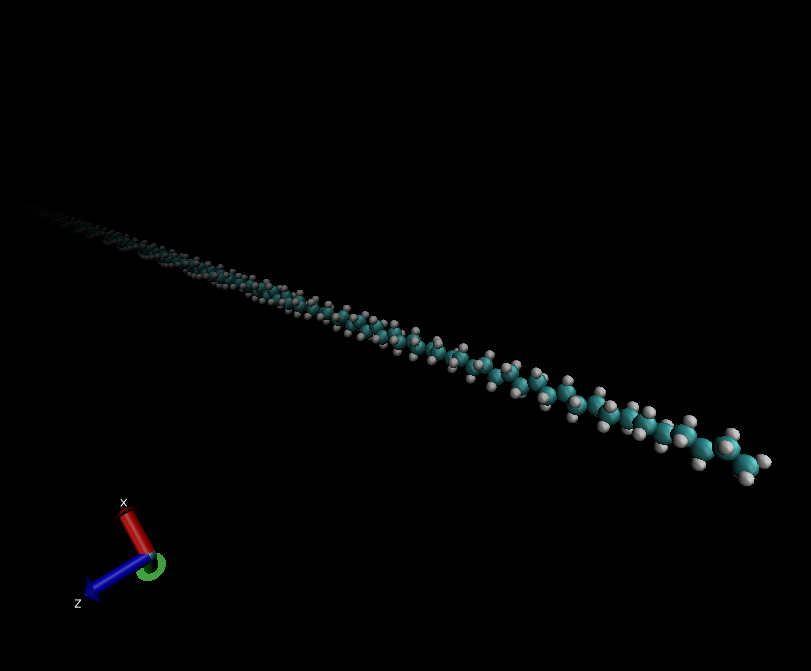
\includegraphics[keepaspectratio,alt={Initial Configuration}]{./img/serial_geweke/VMD_serial_geweke_initial_geometry.png}}
\emph{Fig 1. Initial configuration of the 500-carbon linear polymer
molecule with explicit hydrogens at 300K.}

\pandocbounded{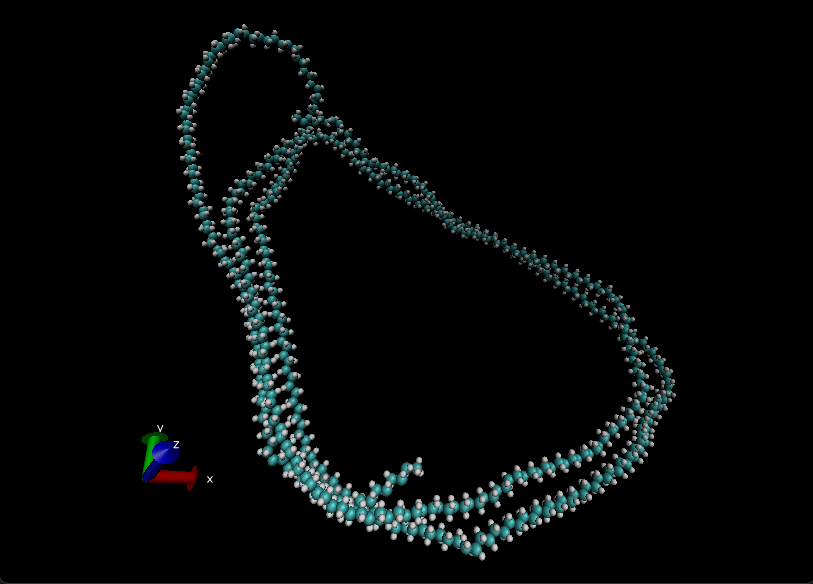
\includegraphics[keepaspectratio,alt={Final Configuration}]{./img/serial_geweke/VMD_serial_geweke_final_geometry.png}}
\emph{Fig 2. Final configuration of the 500-carbon linear polymer
molecule with explicit hydrogens at 300K.}

The python plotting scripts were rewritten to seamlessly stitch these
separate equilibration \& production outputs together across a
time-demarcation boundary:

\paragraph{\texorpdfstring{\textbf{Radius of Gyration \& End-to-End
Sequence (Equilibration \&
Production)}}{Radius of Gyration \& End-to-End Sequence (Equilibration \& Production)}}\label{radius-of-gyration-end-to-end-sequence-equilibration-production}

The polymer begins in an ultra-extended 500-Carbon length chain with
fixed 15-degree dihedrals (\(R_g \approx 200\) Å, \(R_{ee} \approx 600\)
Å), but the random MC modifications rapidly introduce folds. The Geweke
algorithm successfully caught the structural collapse around 3.9 million
steps (denoted by the vertical dashed demarcation line). Everything to
the right of the dashed line behaves exactly as a natural random coil
distribution with stable radial bounds.

\begin{figure}
\centering
\pandocbounded{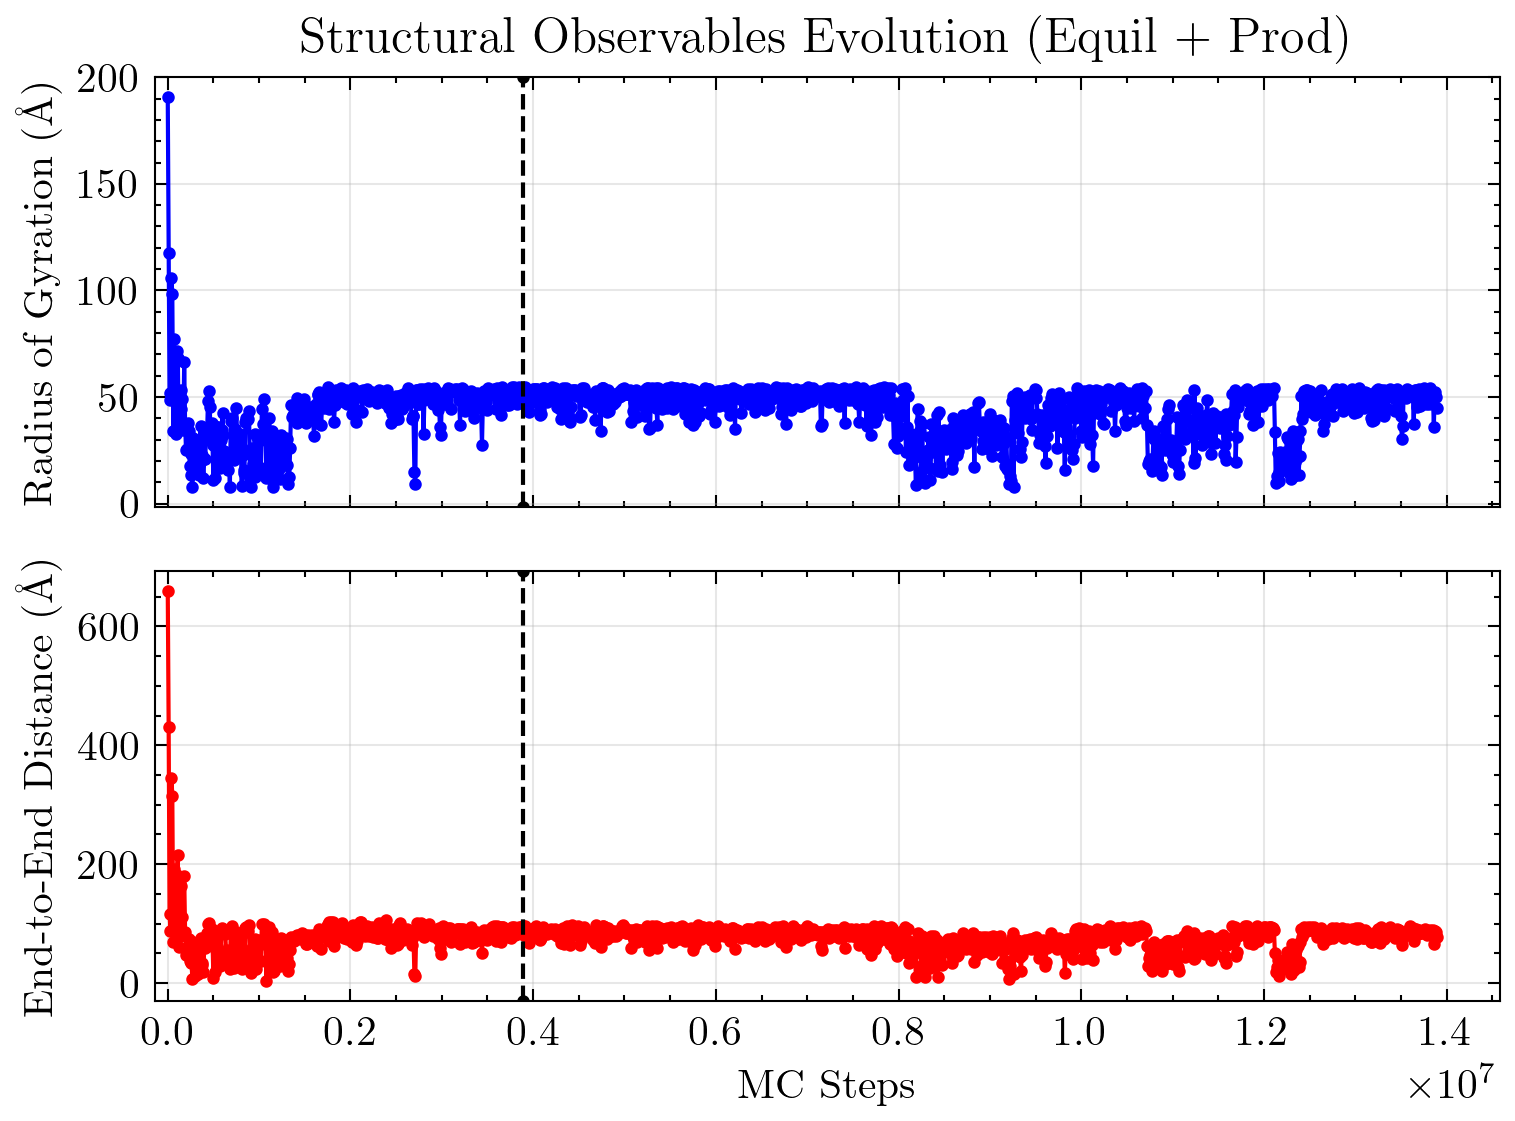
\includegraphics[keepaspectratio,alt={Evolution of Gyration}]{./img/serial_geweke/observables_evolution_500_4_10000000_300.00.png}}
\caption{Evolution of Gyration}
\end{figure}

\paragraph{\texorpdfstring{\textbf{Energy Evolution (Equilibration \&
Production)}}{Energy Evolution (Equilibration \& Production)}}\label{energy-evolution-equilibration-production}

The initial massive spike down for the Lennard-Jones (LJ) energy clearly
captures the steric clash resolving as the linear atoms drift off the
fixed 15-degree axis. Following the Geweke demarcation line at
\textasciitilde3.9M steps, the Total Energy securely flatlines near
\(50\) kcal/mol, mathematically verifying the conformation search has
truly relaxed.

\begin{figure}
\centering
\pandocbounded{
\includegraphics[keepaspectratio,alt={Energy Evolution}]{./img/serial_geweke/energy_evolution_500_4_10000000_300.00.png}}
\caption{Energy Evolution}
\end{figure}

\paragraph{\texorpdfstring{\textbf{Torsional Distribution (Pure
Production)}}{Torsional Distribution (Pure Production)}}\label{torsional-distribution-pure-production}

Plotting the torsional geometry using \emph{only} the production
results, the distribution favors values near \(0\) rad (trans). While
the distribution should \emph{theoretically} mimic the OPLS-AA
potential, the results show a deviation due to the simulation's
preference towards lowering the steric resistance (LJ interactions) over
the total energy. If the latter were preferred, the polymer wouldn't
coil; it would elongate as in the initial conformation.

\begin{figure}
\centering
\pandocbounded{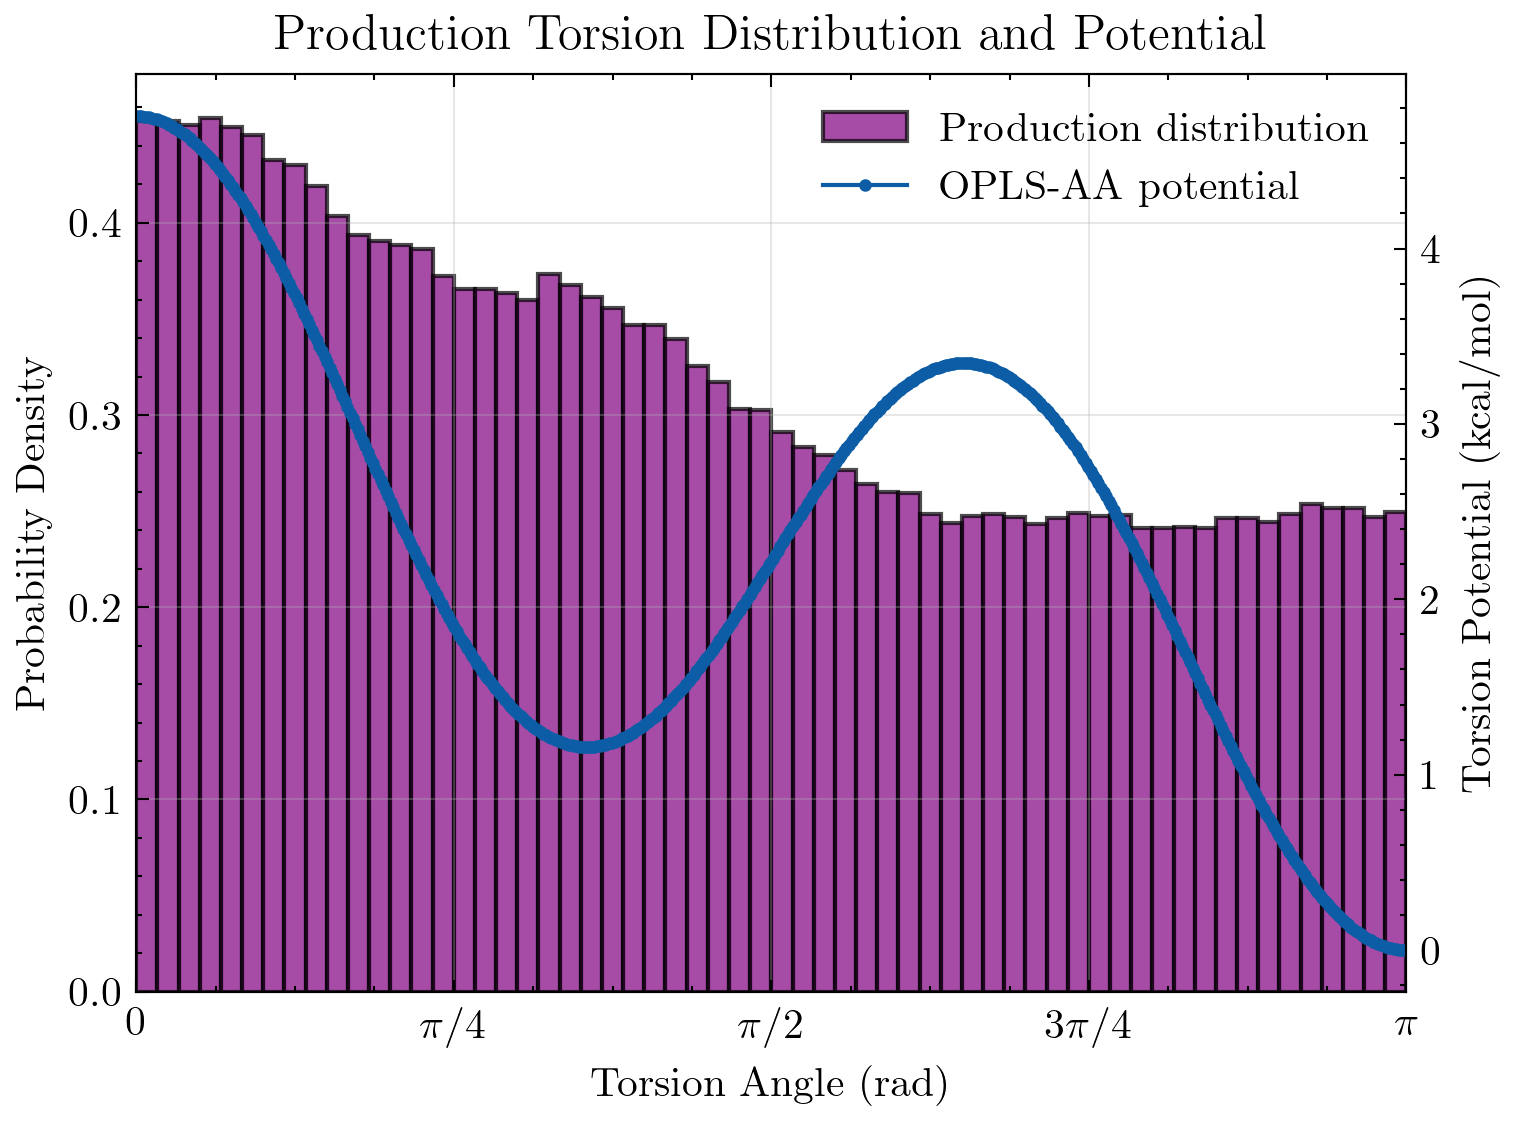
\includegraphics[keepaspectratio,alt={Torsional Distributions}]{./img/serial_geweke/torsion_distribution_500_4_10000000_300.00.png}}
\caption{Torsional Distributions}
\end{figure}

\textbf{Why does the polymer coil instead of staying elongated?}

In these specific simulations there is also a competition between
entropy and energy. As we simulate at 300K, the entropic contribution to
the total energy is significant. Considering entropy is proportional to
the number of available microstates, combined with the probablistic
nature of MCMC simulations, the probability of the chain staying at an
optimal low energy state is overridden by the subjection to a 300K
temperature environment. As such, the polymer coils as it attempts to
find an equilibrium between lowering the energy and getting to a high
entropy state.

\emph{\textbf{Why doesn't the torsional distribution follow the
potential?}}

\textbf{Oliwier to write a note about exclusion of LJ for 1-4 w C, 1-5/6
with H}

Here is why your simulation heavily favors \(0\) radians (a cis-like
geometry) despite the standard theoretical TraPPE/OPLS polynomial
assigning it the highest energy (\(\sim +4.755 \text{ kcal/mol}\)):

\begin{enumerate}
\def\labelenumi{\arabic{enumi}.}
\item
  \textbf{Exclusion of the 1-4 Steric Repulsion}

  The primary physical effect that prevents polymer chains from curling
  back onto themselves to form an exact \(0\) torsion angle is the
  extreme steric clash between atoms located across the exact bond,
  which are a distance of 1-4 bonds apart. If we look at how topology is
  mapped in energy\_all\_atoms.f90, we see this logic:

\begin{Shaded}
\begin{Highlighting}[]
\CommentTok{! If atoms are attached to carbons separated by fewer than 4 bonds, exclude LJ}
\KeywordTok{if}\NormalTok{ (}\BuiltInTok{abs}\NormalTok{(backbone\_pos(i) }\KeywordTok{{-}}\NormalTok{ backbone\_pos(j)) }\OperatorTok{\textless{}} \DecValTok{4}\NormalTok{) }\KeywordTok{then}
\NormalTok{  is\_excluded(i, j) }\KeywordTok{=} \ConstantTok{.true.}
\KeywordTok{end if}
\end{Highlighting}
\end{Shaded}

  This is a standard molecular mechanics trick since the effective
  torsional potentials (opls\_c1, opls\_c2, etc.) supposedly absorb the
  1-4 interactions. However, by blindly turning is\_excluded = .true.
  for all Hydrogen-based interactions separated by fewer than 4 bonds,
  the massive van-der-Waals repulsive core of the explicit Hydrogen
  atoms across the bond is mathematically completely ignored by the
  simulation.
\item
  \textbf{Massive 1-5+ Lennard-Jones Attraction}

  Because the repulsive boundary is artificially turned off, the
  simulation's MC engine evaluates the energy of the geometry entirely
  based on how well it can compact the rest of the chain.

  When explicit hydrogens are included, a highly coiled and overlapped
  structure (which equates to consecutive \(\sim 0\) torsion angles)
  brings the 1-5, 1-6, and 1-n explicit hydrogens into perfectly
  contiguous contact. This dense globule packing results in massive
  Lennard-Jones attractive energy (from slipping perfectly into the
  \(2^{1/6}\sigma\) energy well across hundreds of interatomic pairs).

  Summary of the Physics: The simulation discovers that the dense
  stacking ``reward'' of collapsing dozens of explicit Hydrogens far
  exceeds the purely mathematical \(\sim +4.7\) kcal/mol torsional
  ``penalty'' of having \(\phi\) near \(0\). Since the algorithm
  utilizes the Metropolis criterion purely on the Total Energy (E\_tot =
  E\_lj + E\_tors), it continuously aggregates toward the \(0\) radian
  well.

  If you eventually decide to expand the precision of this simulation,
  introducing a standard scaling rule mechanism like a scale\_14 = 0.5
  modifier for standard 1-4 Lennard-Jones explicit interactions inside
  the delta\_energy function, instead of absolute exclusion, would
  rapidly restore the local minimum clusters expected naturally back to
  your diagram!
\end{enumerate}

\subsection{Parallelization
Techniques}\label{parallelization-techniques}

\subsubsection{Independent Replicas}\label{independent-replicas}

\begin{itemize}
\tightlist
\item
  \textbf{Itxaso to stitch}
\end{itemize}

\subsubsection{Orchestrator Initial Config Read \&
Broadcast}\label{orchestrator-initial-config-read-broadcast}

\begin{itemize}
\tightlist
\item
  \textbf{Itxaso to stitch}
\end{itemize}

\subsubsection{Equilibration
Optimization}\label{equilibration-optimization}

Rather than assigning a single worker to equilibrate each configuration
type independently, a group of \texttt{workers\_per\_equil} MPI workers
is assigned to each configuration type simultaneously. Each worker
starts from the same initial geometry but with a different random seed
(\texttt{rng\_seed\ +\ rank\ ×\ 104729}), ensuring that trajectories
immediately diverge and explore distinct regions of conformational
space.

Every \texttt{sync\_interval} MC steps, a synchronisation protocol is
executed: each worker sends its current energy and \(R_g\) to the
master, which selects the most representative configuration via a
Boltzmann-weighted roulette wheel and broadcasts those coordinates back
to the non-winning workers in the group. The winning worker continues
its trajectory uninterrupted, preserving the best conformational path
found so far.

\paragraph{Replica Selection: Boltzmann Roulette
Wheel}\label{replica-selection-boltzmann-roulette-wheel}

At each synchronisation point, the master assigns a statistical weight
to each replica \(i\) based on its total energy \(E_i\):

\[w_i = \exp\!\left(-\frac{E_i - E_{\min}}{k_B \, T_{\text{virt}}}\right)\]

where \(E_{\min}\) is the lowest energy in the current group and
\(T_{\text{virt}}\) is a virtual temperature --- a purely algorithmic
parameter with no physical meaning. It controls how aggressively
low-energy replicas are favoured:

\begin{itemize}
\tightlist
\item
  \(T_{\text{virt}} \to 0\): deterministic selection of the
  minimum-energy replica.
\item
  \(T_{\text{virt}} \to \infty\): uniform selection, ignoring energies.
\end{itemize}

A uniform random number then samples this distribution via
roulette-wheel selection, and the selected replica's coordinates are
sent to the non-winning workers:

\begin{Shaded}
\begin{Highlighting}[]
\NormalTok{E\_min\_grp }\KeywordTok{=} \FunctionTok{minval}\NormalTok{(grp\_energies)}
\KeywordTok{do}\NormalTok{ w }\KeywordTok{=} \DecValTok{1}\NormalTok{, workers\_per\_equil}
\NormalTok{  grp\_boltz(w) }\KeywordTok{=} \BuiltInTok{exp}\NormalTok{(}\KeywordTok{{-}}\NormalTok{(grp\_energies(w) }\KeywordTok{{-}}\NormalTok{ E\_min\_grp) }\KeywordTok{/}\NormalTok{ (kb }\KeywordTok{*}\NormalTok{ T\_virt))}
\KeywordTok{end do}
\NormalTok{tw }\KeywordTok{=} \FunctionTok{sum}\NormalTok{(grp\_boltz)}
\CommentTok{call random\_number(r\_pick)}
\NormalTok{accum }\KeywordTok{=} \FloatTok{0.0d0}
\NormalTok{best\_local }\KeywordTok{=}\NormalTok{ workers\_per\_equil}
\KeywordTok{do}\NormalTok{ w }\KeywordTok{=} \DecValTok{1}\NormalTok{, workers\_per\_equil}
\NormalTok{  accum }\KeywordTok{=}\NormalTok{ accum }\KeywordTok{+}\NormalTok{ grp\_boltz(w) }\KeywordTok{/}\NormalTok{ tw}
  \KeywordTok{if}\NormalTok{ (r\_pick }\OperatorTok{\textless{}=}\NormalTok{ accum) }\KeywordTok{then}
\NormalTok{    best\_local }\KeywordTok{=}\NormalTok{ w}
    \KeywordTok{exit}
  \KeywordTok{end if}
\KeywordTok{end do}
\end{Highlighting}
\end{Shaded}

\paragraph{MPI Communication Protocol}\label{mpi-communication-protocol}

The synchronisation uses only point-to-point MPI operations
(\texttt{MPI\_Send} / \texttt{MPI\_Recv}) to avoid the need for
temporary communicators or collective operations across worker
subgroups. At each sync point, the master loops over all \(K\) workers
in the active equilibration group:

{\def\LTcaptype{none} % do not increment counter
\begin{longtable}[]{@{}
  >{\raggedright\arraybackslash}p{(\linewidth - 6\tabcolsep) * \real{0.1935}}
  >{\raggedright\arraybackslash}p{(\linewidth - 6\tabcolsep) * \real{0.3548}}
  >{\raggedright\arraybackslash}p{(\linewidth - 6\tabcolsep) * \real{0.1613}}
  >{\raggedright\arraybackslash}p{(\linewidth - 6\tabcolsep) * \real{0.2903}}@{}}
\toprule\noalign{}
\begin{minipage}[b]{\linewidth}\raggedright
Step
\end{minipage} & \begin{minipage}[b]{\linewidth}\raggedright
Direction
\end{minipage} & \begin{minipage}[b]{\linewidth}\raggedright
Tag
\end{minipage} & \begin{minipage}[b]{\linewidth}\raggedright
Content
\end{minipage} \\
\midrule\noalign{}
\endhead
\bottomrule\noalign{}
\endlastfoot
1 & worker → master & \texttt{TAG\_SYNC\_OBS} &
\([E_{\text{total}},\, R_g^2]\) \\
2 & master → worker & \texttt{TAG\_SYNC\_CTRL} &
\texttt{{[}ctrl\_signal,\ best\_local\_idx{]}} \\
3 & worker → master & \texttt{TAG\_EQUIL\_COORDS} & full coordinate
array \\
4 & master → non-winners & \texttt{TAG\_SYNC\_COORDS} & winning
coordinates \\
\end{longtable}
}

Once the Geweke test declares equilibrium, the master saves the
equilibrated geometry to \texttt{../results/equilibrated\_cX.xyz} and
unlocks the 10 production jobs for that configuration type in the task
queue.

\paragraph{Metrics and Methodology}\label{metrics-and-methodology}

This section evaluates the performance of the equilibration optimization
technique compared to the serial baseline. The system studied is
configuration 1, a chain of 500 carbons at \(T = 300\,\text{K}\)
including hydrogens.

Efficiency is evaluated based on the time to reach specific energy
thresholds (\(E_{\text{total}} < 110,\, 100,\text{ and } 90\) kcal/mol).
The speedup is defined as
\(S(w) = \text{Steps}_{\text{serial}} / \text{Steps}_{\text{parallel}}(w)\).

\textbf{Convergence Efficiency and Superlinear Speedup}

The table below summarises the number of MC steps required by different
worker configurations to reach the target energy levels.

{\def\LTcaptype{none} % do not increment counter
\begin{longtable}[]{@{}
  >{\raggedright\arraybackslash}p{(\linewidth - 8\tabcolsep) * \real{0.1392}}
  >{\centering\arraybackslash}p{(\linewidth - 8\tabcolsep) * \real{0.1899}}
  >{\raggedleft\arraybackslash}p{(\linewidth - 8\tabcolsep) * \real{0.2025}}
  >{\centering\arraybackslash}p{(\linewidth - 8\tabcolsep) * \real{0.2025}}
  >{\centering\arraybackslash}p{(\linewidth - 8\tabcolsep) * \real{0.2658}}@{}}
\toprule\noalign{}
\begin{minipage}[b]{\linewidth}\raggedright
Threshold
\end{minipage} & \begin{minipage}[b]{\linewidth}\centering
Workers (\(w\))
\end{minipage} & \begin{minipage}[b]{\linewidth}\raggedleft
Steps Required
\end{minipage} & \begin{minipage}[b]{\linewidth}\centering
Speedup \(S(w)\)
\end{minipage} & \begin{minipage}[b]{\linewidth}\centering
Efficiency \(S(w)/w\)
\end{minipage} \\
\midrule\noalign{}
\endhead
\bottomrule\noalign{}
\endlastfoot
\(E < 110\) kcal/mol & 1 & 590,000 & 1.00 & 1.00 \\
& 2 & 70,000 & 8.43 & 4.21 \\
& 4 & 140,000 & 4.21 & 1.05 \\
& 8 & 50,000 & 11.80 & 1.47 \\
\(E < 100\) kcal/mol & 1 & 1,180,000 & 1.00 & 1.00 \\
& 2 & 350,000 & 3.37 & 1.68 \\
& 4 & 210,000 & 5.62 & 1.40 \\
& 8 & 50,000 & 23.60 & 2.95 \\
\(E < 90\) kcal/mol & 1 & 2,400,000 & 1.00 & 1.00 \\
& 2 & 1,780,000 & 1.35 & 0.67 \\
& 4 & 570,000 & 4.21 & 1.05 \\
& 8 & 160,000 & 15.00 & 1.87 \\
\end{longtable}
}

\pandocbounded{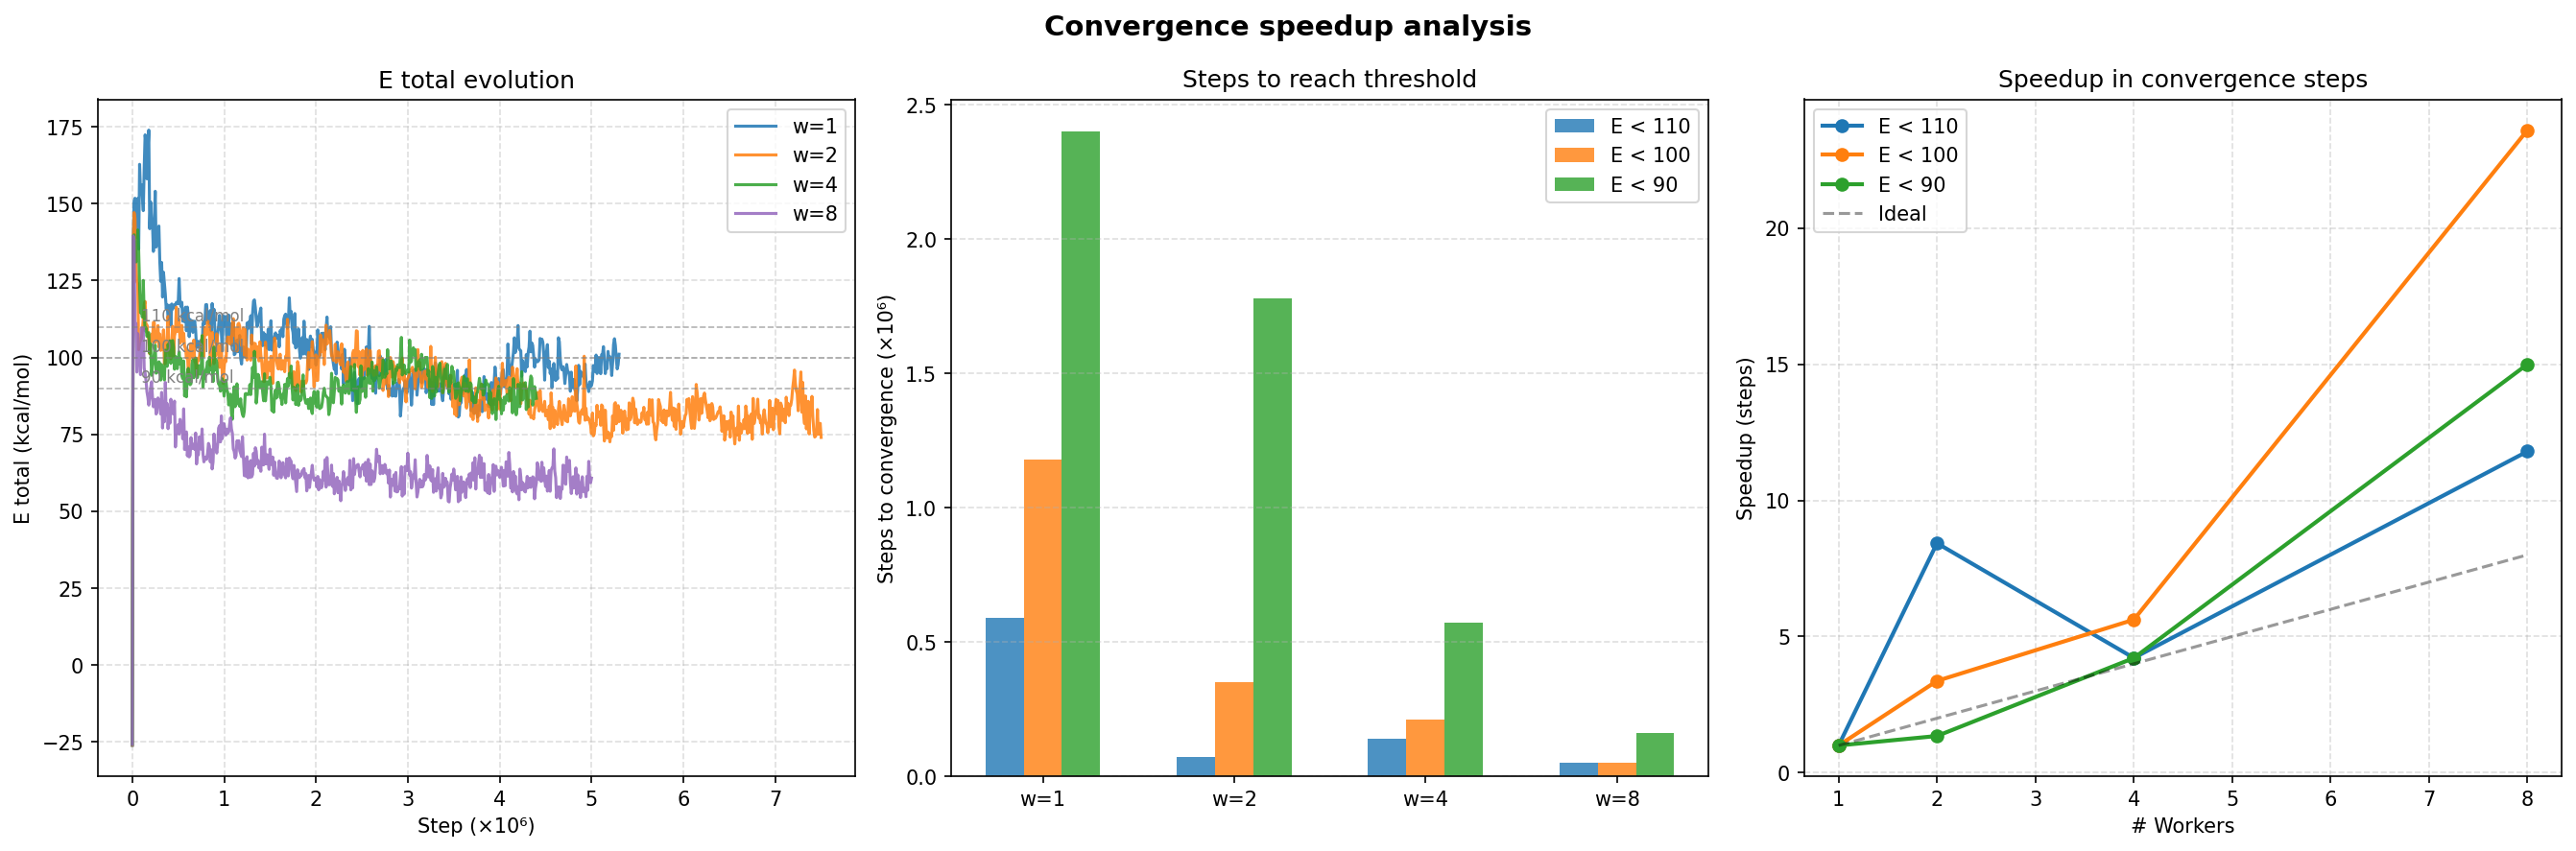
\includegraphics[keepaspectratio,alt={Convergence speedup analysis}]{./Manel/convergence_speedup_equil.png}}
\emph{Convergence speedup analysis. Left: evolution of
\(E_\text{total}\) for each worker configuration. Centre: MC steps
required to reach each energy threshold. Right: speedup \(S(w)\)
relative to the serial run; the dashed line shows ideal linear scaling.}

The results demonstrate a clear superlinear speedup (\(S(w) > w\)) in
almost all parallel configurations. This phenomenon is a direct
consequence of the collaborative sampling strategy implemented via the
Boltzmann roulette wheel.

In the serial run, the polymer chain often becomes trapped in metastable
states (local energy minima). The parallel implementation, by
maintaining a population of \(w\) independent trajectories,
significantly increases the probability that at least one replica
discovers a more favorable region of the phase space. Once a
lower-energy conformation is found, the synchronization protocol
``rescues'' the rest of the population, broadcasting the winning
coordinates to all workers. This creates a collective escape mechanism
that reduces the number of steps required to converge by a factor far
greater than the number of processors.

For instance, at the 100 kcal/mol threshold, the 8-worker group reaches
the target in only 50,000 steps, compared to the 1.18 million steps
required by the serial run, resulting in a speedup of \textbf{23.60×}.

We also observe stochastic fluctuations typical of Monte Carlo methods,
such as the anomalous efficiency at \(w=2\) for the 110 kcal/mol
threshold. As the energy targets become more stringent (90 kcal/mol),
the speedup values tend to stabilize, as finding further conformational
improvements becomes more difficult even for a larger population.

\subsubsection{Energy Calculations}\label{energy-calculations}

\paragraph{\texorpdfstring{\texttt{compute\_total\_energy}}{compute\_total\_energy}}\label{compute_total_energy}

The dominant cost in \texttt{compute\_total\_energy} is the
\(\mathcal{O}(N^2)\) double loop over non-bonded LJ pairs. Each
iteration is independent --- it reads a pair of coordinates, evaluates
\texttt{lj\_pair\_energy}, and adds to a running sum --- which makes it
a natural fit for OpenMP worksharing. The outer loop over \texttt{i} is
distributed across threads with \texttt{!\$omp\ parallel\ do}, with the
inner index \texttt{j}, the squared distance \texttt{r2}, and the
dihedral cosine \texttt{cos\_phi} declared private to prevent
cross-thread interference. The global accumulators \texttt{e\_lj} and
\texttt{e\_tors} are aggregated safely with a \texttt{reduction(+:...)}
clause.

The two loops inside the subroutine have different iteration structures
and were scheduled accordingly. The LJ pair loop has a triangular
iteration space (the inner bound depends on \texttt{i}), so
\texttt{schedule(dynamic,\ 10)} is used to prevent faster threads from
sitting idle while slower ones finish large inner loops. The torsional
loop over the carbon backbone is uniform in length and uses the default
static scheduling, which has lower overhead when the workload is
balanced.

Both parallel regions are wrapped in an \texttt{if(omp\_total\_energy)}
runtime guard, which is set from the input file. This allows the same
binary to run in purely serial mode during development or lightweight
tests without any code changes.

\paragraph{\texorpdfstring{\texttt{delta\_energy}}{delta\_energy}}\label{delta_energy}

The \texttt{delta\_energy} subroutine is the true bottleneck of the MC
loop --- it is called once per accepted or rejected move, millions of
times per simulation. The key algorithmic feature here is the dynamic
partitioning of atoms into \texttt{fixed\_list} and \texttt{moved\_list}
at the start of each call. Only cross-interactions between fixed and
moved atoms can have changed during a pivot, so the LJ loop processes
exclusively those pairs rather than the full \(\mathcal{O}(N^2)\) set.

The two nested loops over \texttt{f} (fixed) and \texttt{m} (moved) form
a perfectly rectangular iteration space, which makes
\texttt{collapse(2)} effective: it merges both loops into a single flat
range of \texttt{n\_fixed\ ×\ n\_moved} iterations and distributes them
evenly across threads. Since pivot moves near chain ends move very few
atoms, spawning threads for a handful of pairs would cost more than it
saves. The parallel block is therefore gated by
\texttt{if(omp\_delta\_energy\ .and.\ (n\_fixed\ *\ n\_moved\ \textgreater{}\ 1000))},
ensuring parallelization is only activated when the workload genuinely
justifies it.

\paragraph{Benchmarking Code}\label{benchmarking-code}

To quantify the effect of thread count on both energy routines, a
dedicated benchmark program \texttt{main\_bench\_total.f90} was written.
It performs 10,000 back-to-back calls to \texttt{compute\_total\_energy}
for a given chain size and reports the wall time via MPI\_Wtime. Two
shell scripts automate the full benchmark sweeps:
\texttt{4.run\_omp\_total\_test.sh} compiles and runs the benchmark
binary across thread counts of 1, 2, 3, and 4 for chain sizes of 20, 50,
100, and 500 carbons, writing results to a CSV in
\texttt{results/bench\_omp\_total/}.

\texttt{5.run\_omp\_delta\_test.sh} follows the same structure but
targets \texttt{delta\_energy} by running full 1M-step MC simulations
via \texttt{main\_parallel\_replicas.x} and extracting wall time from
the CPU output files. Both scripts are written for the
\texttt{cerqt01.q} cluster queue and load the appropriate MPI module.
The results are plotted by \texttt{plot\_benchmarks.py}, which reads
both CSVs and produces per-chain-size scaling plots as PDFs.

\textbf{Oliwier to add images/results/analysis, plus talk about
benchmarking being affected by randomness}

\paragraph{SIMD Exploration}\label{simd-exploration}

An attempt was made to additionally exploit single-core SIMD
vectorization on the \texttt{lj\_pair\_energy} function using the
\texttt{!\$omp\ declare\ simd} directive. The idea was to generate a
vectorized variant of the function callable from an
\texttt{!\$omp\ simd}-annotated inner loop, allowing each thread to
process multiple atom pairs simultaneously using AVX registers. In
practice, activating this required structural changes to
\texttt{delta\_energy} that conflicted with the existing threading
design: the \texttt{collapse(2)} clause and the inner-loop cycle on
\texttt{is\_excluded} are incompatible with SIMD regions, and removing
them to support vectorization degraded the thread load balancing that
\texttt{collapse(2)} provides. Given that the OpenMP threading was the
primary parallelization goal, the SIMD experiment was abandoned and the
directive was removed from the code. It remains a direction worth
revisiting, particularly if the pair loops were refactored to use
pre-filtered pair lists that eliminate the exclusion branch entirely.

\subsubsection{Ensemble Averaging}\label{ensemble-averaging}

Moving to an Orchestrator-Worker (Star) topology helped with the
transition of the serial environment to a dynamically balanced parallel
framework with OpenMPI. It achieves maximum CPU utilization by ensuring
free workers are constantly assigned tasks until the simulation is
complete.

Although this architechure adds overhead by requiring a single core to
abstain from participating in the simulation's calculations, the
orchestrator node performs the administrative tasks such as the initial
file reading as well as organizing and distributing the workload. This
relies upon tags being sent between the nodes to coordinate the
simulation.

\begin{Shaded}
\begin{Highlighting}[]
  \CommentTok{! MPI Tags}
  \DataTypeTok{integer}\NormalTok{, }\DataTypeTok{parameter} \DataTypeTok{::}\NormalTok{ TAG\_REQUEST\_WORK }\KeywordTok{=} \DecValTok{1}
  \DataTypeTok{integer}\NormalTok{, }\DataTypeTok{parameter} \DataTypeTok{::}\NormalTok{ TAG\_DO\_EQUIL     }\KeywordTok{=} \DecValTok{2}
  \DataTypeTok{integer}\NormalTok{, }\DataTypeTok{parameter} \DataTypeTok{::}\NormalTok{ TAG\_DO\_PROD      }\KeywordTok{=} \DecValTok{3}
  \DataTypeTok{integer}\NormalTok{, }\DataTypeTok{parameter} \DataTypeTok{::}\NormalTok{ TAG\_WAIT         }\KeywordTok{=} \DecValTok{4}
  \DataTypeTok{integer}\NormalTok{, }\DataTypeTok{parameter} \DataTypeTok{::}\NormalTok{ TAG\_DIE          }\KeywordTok{=} \DecValTok{5}
  \DataTypeTok{integer}\NormalTok{, }\DataTypeTok{parameter} \DataTypeTok{::}\NormalTok{ TAG\_EQUIL\_DONE   }\KeywordTok{=} \DecValTok{6}
  \DataTypeTok{integer}\NormalTok{, }\DataTypeTok{parameter} \DataTypeTok{::}\NormalTok{ TAG\_PROD\_DONE    }\KeywordTok{=} \DecValTok{7}
\end{Highlighting}
\end{Shaded}

First, the simulation is cleanly segregated into phases where the
\textbf{Orchestrator Node} acts as a central dispatcher:

\begin{Shaded}
\begin{Highlighting}[]
      \KeywordTok{do} \KeywordTok{while}\NormalTok{ (completed\_prods }\OperatorTok{\textless{}} \FunctionTok{size}\NormalTok{(prod\_queue))}
         \CommentTok{! Wait for any worker to finish its task and ask for more}
         \KeywordTok{call}\NormalTok{ MPI\_Recv(msg, }\DecValTok{1}\NormalTok{, MPI\_INTEGER, MPI\_ANY\_SOURCE, MPI\_ANY\_TAG,}\CommentTok{ MPI\_COMM\_WORLD, status, ierr)}
\NormalTok{         sender }\KeywordTok{=}\NormalTok{ status(MPI\_SOURCE)}
\NormalTok{         tag\_recvd }\KeywordTok{=}\NormalTok{ status(MPI\_TAG)}
\end{Highlighting}
\end{Shaded}

\begin{itemize}
\tightlist
\item
  \texttt{MPI\_Recv}: The orchestrator lies in wait for any incoming
  communication from the worker nodes.
\item
  \texttt{MPI\_ANY\_SOURCE}: Instead of statically assigning jobs to
  specific processors up-front, the orchestrator listens to the
  \emph{entire pool} of available cores. As soon as a worker node
  finishes its current 1-million-step job, it pings the orchestrator,
  which instantly deploys the next job from the queue directly to that
  specific idle worker, ensuring optimal resource utilization.
\item
  \textbf{Staged Execution}: By cleanly separating the logic phases, the
  orchestrator refuses to load the 10 production jobs into the queue
  until the prerequisite equilibration run officially finishes. The
  moment equilibration is met, jobs pop into the queue and cores are
  reused instantly, guaranteeing no resources are ever permanently
  ``blocked'' waiting in idle lines.
\end{itemize}

Once a worker has sent an incoming communication signal back to the
orchestrator, the orchestrator checks the tag and executes the
appropriate logic:

\begin{Shaded}
\begin{Highlighting}[]
         \KeywordTok{if}\NormalTok{ (tag\_recvd }\OperatorTok{==}\NormalTok{ TAG\_EQUIL\_DONE) }\KeywordTok{then}
           \CommentTok{! ... (Orchestrator caches the equilibrated .xyz coordinates and unlocks the production queue)}
         \KeywordTok{else if}\NormalTok{ (tag\_recvd }\OperatorTok{==}\NormalTok{ TAG\_PROD\_DONE) }\KeywordTok{then} 
           \CommentTok{! ... (Orchestrator tallies the completed production run)}
         \KeywordTok{end if}

         \CommentTok{! If jobs remain in the queue, immediately deploy the next one to the \textquotesingle{}sender\textquotesingle{}}
         \KeywordTok{if}\NormalTok{ (jobs\_assigned }\OperatorTok{\textless{}} \FunctionTok{size}\NormalTok{(prod\_queue)) }\KeywordTok{then}
            \KeywordTok{call}\NormalTok{ MPI\_Send(TAG\_DO\_PROD, }\DecValTok{1}\NormalTok{, MPI\_INTEGER, sender, TAG\_DO\_PROD, MPI\_COMM\_WORLD, ierr)}
\end{Highlighting}
\end{Shaded}

\begin{itemize}
\tightlist
\item
  \texttt{MPI\_Send}: Deploys the next instruction array sequentially to
  whichever Worker ID is populated in the \texttt{sender} variable.
\item
  \texttt{TAG\_DO\_PROD}: An statically assigned integer tag that tells
  the receiving Worker process exactly which computational sub-routine
  to pivot into.
\end{itemize}

The benefits of this star topology combined with phased execution of
equilibration runs followed by production runs is compared below to the
serial version of the program. As the number of dynamic active nodes
increases, the time to complete 10-million MC Steps decreases, albeit
non-ideally:

\pandocbounded{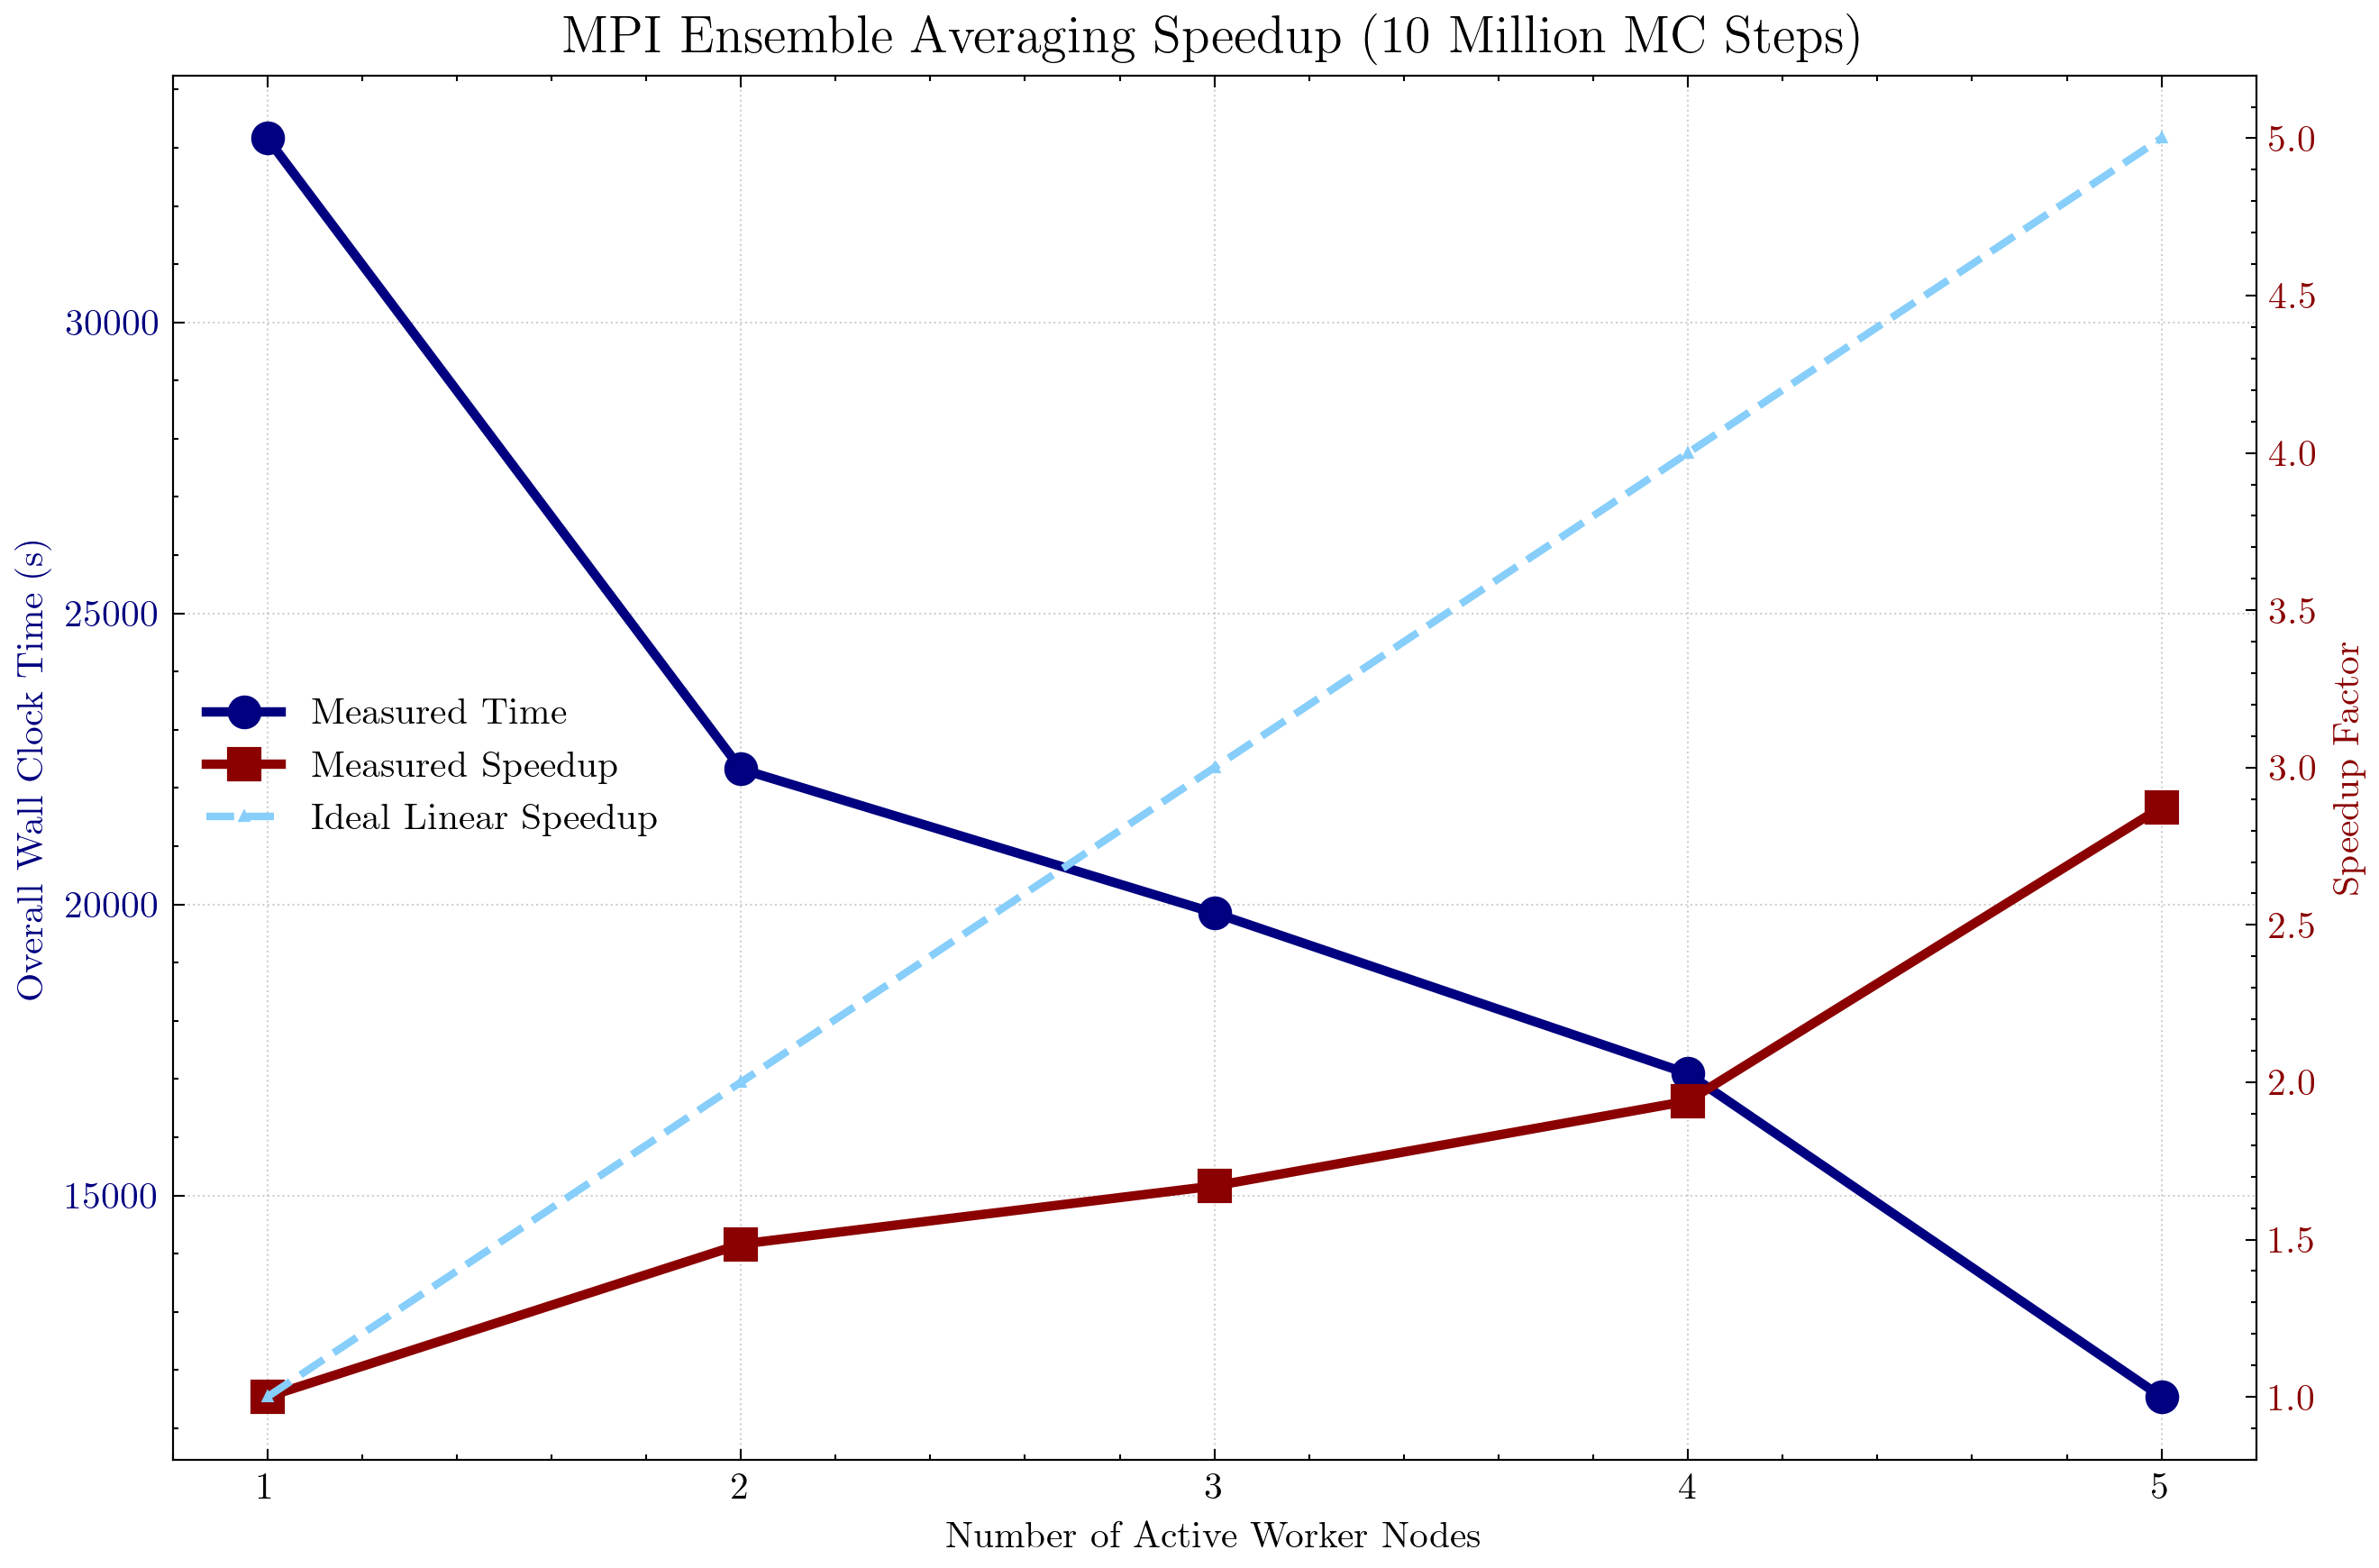
\includegraphics[keepaspectratio,alt={MPI Parallel Speedup Analysis}]{img/parallel_star_speedup_plot.png}}
\emph{Fig. x: Comparing timing \& efficiency of Ensemble Averaging with
various core count to Serial production run}

Simply adding more cores does not result in a perfectly linear speedup.
This can be attributed to parallelization overhead plus device hardware
bottlenecks. The most efficient use of cores is found in factors of 10
(2 \& 5 cores), in which cases all worker nodes are participating in the
final group of remaining 1M MCS steps. The non-factors of 10 could see
performance improvements with the addition of a dynamic algorithm that
determines how many steps are left once there are fewer 1M MCS jobs
remaining than cores participating. This would eliminates worker
``dead-time'' towards the end of the production run.

\subsubsection{Trajectory Analysis}\label{trajectory-analysis}

\subsection{Serial vs Parallel
Performance}\label{serial-vs-parallel-performance}

The serial code was run on a single core of an Intel Core i7-11800H
processor, taking 8 hours, 18 minutes, and 31.91 seconds. The parallel
code was run on 4 cores of the same processor, taking \_\_ hours, \_\_
minutes, and \_\_ seconds. The parallel code was run using the
\texttt{mpirun} command with the \texttt{-np\ 4} option.

\subsection{Conclusion}\label{conclusion}

\subsubsection{Computer Simulation vs Real-World
Results}\label{computer-simulation-vs-real-world-results}

While this Monte Carlo simulation successfully modeled the
conformational sampling of a polymer chain, it is important to recognize
the limitations when comparing theoretical calculations to real-world
experimental results.

\begin{itemize}
\tightlist
\item
  By employing the OPLS-AA and TraPPE-UA force fields, we gain robust
  mathematical approximations of energy landscapes; however, these
  empirical potentials cannot fully capture the dynamic complexities of
  real-world solvent interactions or subtle quantum effects.
\item
  The isolation of a single polymer chain within the simulation neglects
  the significant impact of intermolecular forces and environmental
  factors that would be present in a real-world scenario.
\item
  Additionally, our exclusion of standard 1-4 steric repulsions skewed
  the expected torsional distribution towards a cis-like geometry,
  highlighting how algorithmic approximations can yield results that
  diverge from established empirical physical behaviors.
\end{itemize}

\subsubsection{Nonlinearity of Parallel
Speedup}\label{nonlinearity-of-parallel-speedup}

One of the key observations from our performance analysis is that
parallelization rarely translates evenly into a 1:1, linear speedup. In
a perfect scenario, assigning four cores would make the code run four
times faster. However, as seen in our MPI benchmarks, adding more
workers inherently introduces communication overhead. The time required
for the orchestrator to pass messages, synchronize coordinates during
ensemble sampling, and track dynamic convergence tests gradually eats
into the raw processing speed. At certain hardware boundaries,
communication bottlenecks and competition for physical system resources
make additional core count benefits negligible.

\subsubsection{Navigating Resource
Utilization}\label{navigating-resource-utilization}

Combining multiple High-Performance Computing (HPC) methodologies---like
MPI and OpenMP---offered profound acceleration capabilities, but as
stated in the
\href{./EIA_Project2026_Report_GroupII.md\#parallelization-with-mpi--openmp}{Parallelization
with MPI \& OpenMP} section, requires careful resource management to
prevent oversubscription. Breaking up the simulation workflow into
phases proved to be a critical step in reusing resources and limiting
the system size required to run the program.

\subsubsection{HPC Optimization}\label{hpc-optimization}

Ultimately, achieving high performance is not simply a matter of
checking if a particular parallel processing technique outpaces its
serial counterpart, rather it requires a coordinated benchmarking
strategy. Optimizing an HPC code ecosystem demands that we carefully
evaluate how different techniques overlap and complement one another.
Were this a commercial or funded research project, benchmarking the
performance of the various technique combinations (and against the
system hardware available) would be prudent.

\subsection{Summary of the Combined Parallelized Program
Logic}\label{summary-of-the-combined-parallelized-program-logic}

\begin{figure}
\centering
\pandocbounded{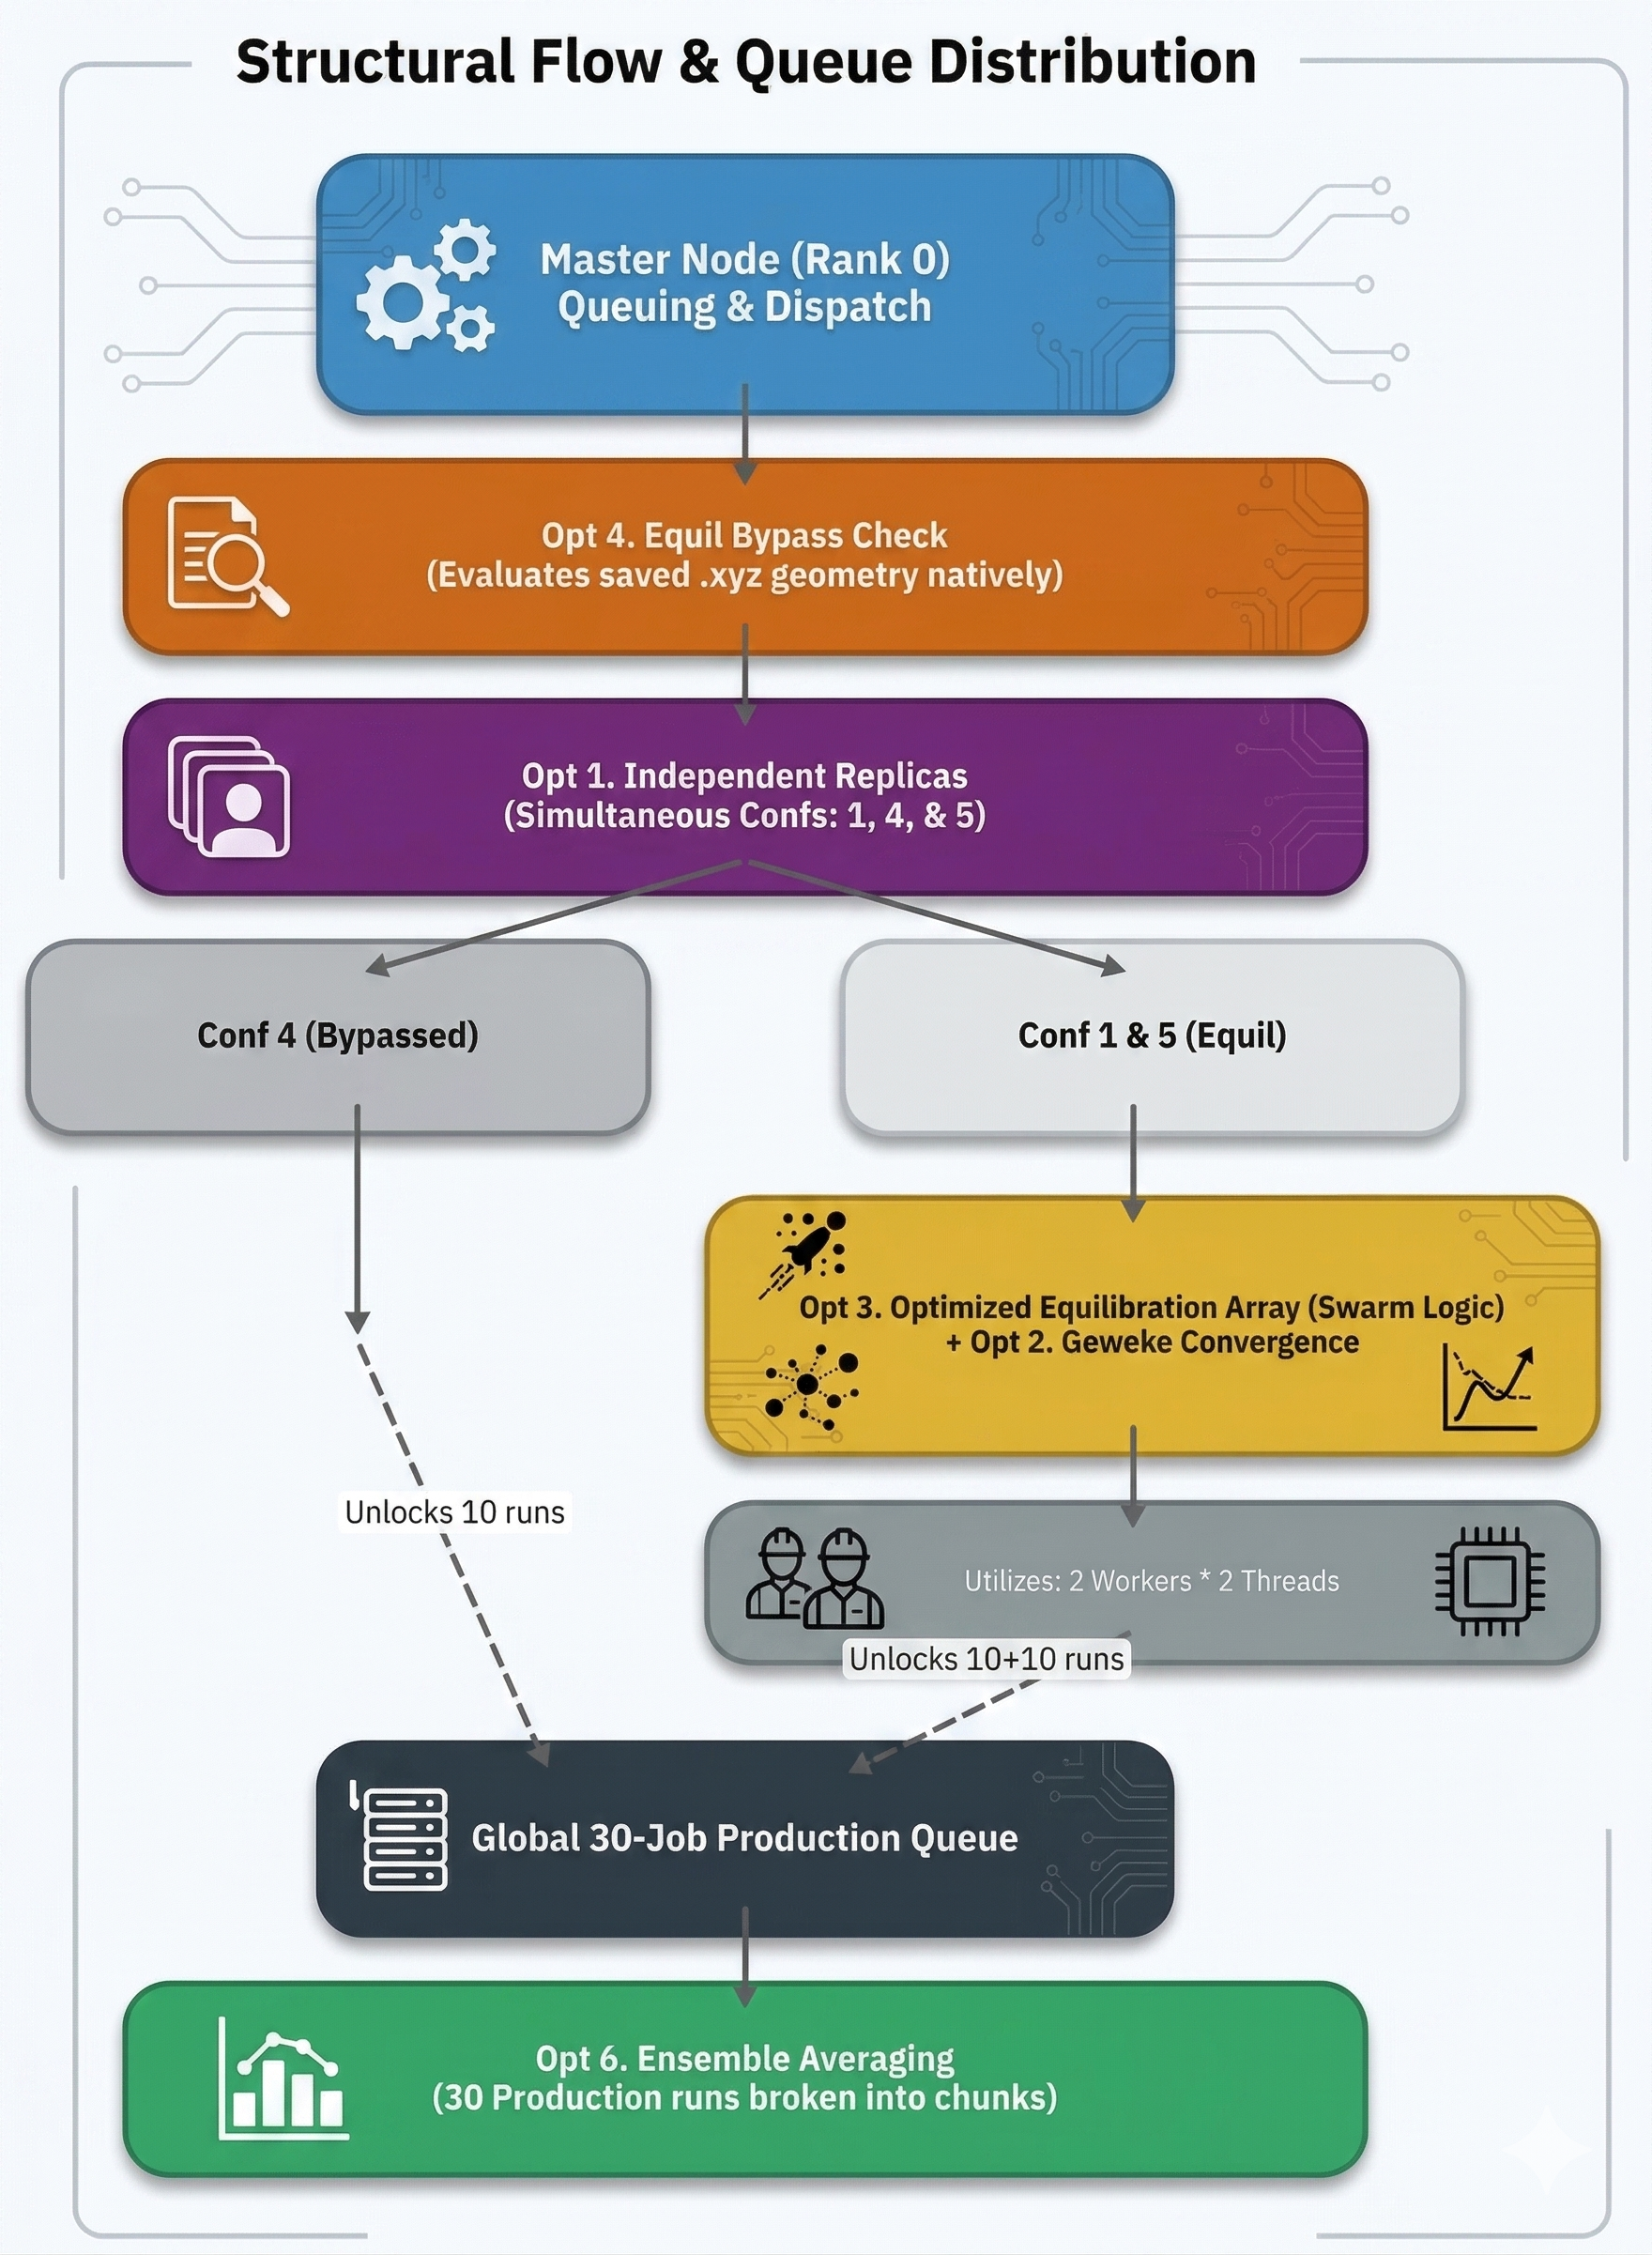
\includegraphics[keepaspectratio,alt={Resouce Utilization}]{./img/ParallelProcessing_ResourceUtilization.png}}
\caption{Resouce Utilization}
\end{figure}

The diagram above illustrates our parallel processing architecture,
which leverages a central Master Node to efficiently orchestrate tasks
across the system. With combined optimization and parallelization
techniques, a possible workflow functions as follows:

\begin{itemize}
\tightlist
\item
  The Master Node checks if an equilibrated geometry already exists,
  allowing it to bypass the computationally heavy equilibration phase
  for previously processed configurations (such as Conf 4, which
  immediately unlocks its production runs).
\item
  For new configurations (like Confs 1 and 5), the system simultaneously
  deploys independent replicas.
\item
  These replicas utilize a collaborative swarm logic, aided by the
  Geweke Convergence test running on 2 workers with 2 threads each, to
  dynamically find equilibrium as fast as possible.
\item
  Since an equilibrated geometry for conformation type 4 is already
  supplied, the 2 workers with their 2 OpenMP threads each are
  immediately available to assist in the production runs for that
  configuration.
\item
  Meanwhile equilibration completes for conformations 4 \& 5, and those
  workers become available to start assisting in the remaining jobs from
  the shared 30-job global production queue.
\end{itemize}

Total core count for this scenario (default when
\texttt{run\_parallel.qsub} is invoked) is \textbf{13 cores}: -
\textbf{1} Master Node (\textbf{1 core}) - 2 Workers each running a
Conformation Equilibration - Each of these workers takes 2 cores for
Swarm Logic - Each node calculates energy via 2 OpenMP threads
(\(2x2x2=\) \textbf{8 cores}) - 2 Workers immediately start production
runs on equilibration-bypassed conformation \#4. (\emph{Why 2? The
system opts to utilize the same number of workers for a bypassed
configuration as it would a swarm-logic equilibration.}) - These
workers' energy calculations are threaded with OpenMP (\(2x2=\)
\textbf{4 cores}) - When the equilibration phase is done for
conformations 1 \& 5, those workers are reassigned unfinished chunks of
the production queue, \emph{reusing the CPU resources}, 4 cores per
conformation. (\textbf{+0 cores}) - As workers finish their subtasks,
they inform the orchestrator, receiving any pending jobs from the global
queue until all 30 production jobs are completed. (\textbf{+0 cores})

\subsection{References}\label{references}

\begin{itemize}
\tightlist
\item
  {[}1{]} Roy, V. (2020). Convergence Diagnostics for Markov Chain Monte
  Carlo. \emph{Annual Review of Statistics and Its Application}, 7,
  387--412. https://doi.org/10.1146/annurev-statistics-031219-041300
\item
  {[}2{]} \textbf{Oliwier to send - used in TraPPE-UA section}
\item
  {[}3{]} \textbf{Oliwier to send - used in OPLS-AA section}
\end{itemize}

\end{document}
